%
% A header that lets you compile a chapter by itself, or inside a larger document.
% Adapted from http://stackoverflow.com/questions/3655454/conditional-import-in-latex
%
%
%Use \inbpdocument and \outbpdocument in your individual files, in place of \begin{document} and \end{document}. In your main file, put in a \def \ismaindoc {} before including or importing anything.
%
% David Duvenaud
% June 2011
% 
% ======================================
%
%


\ifx\ismaindoc\undefined
	\newcommand{\inbpdocument}{
		\def \ismaindoc {}
		% Use this header if we are compiling by ourselves.
		\documentclass[a4paper,11pt,authoryear,index]{common/PhDThesisPSnPDF}
		
%\usepackage{draftwatermark}
%\SetWatermarkLightness{0.95}

% ******************************************************************************
% ****************************** Custom Margin *********************************

% Add `custommargin' in the document class options to use this section
% Set {innerside margin / outerside margin / topmargin / bottom margin}  and
% other page dimensions

\ifsetMargin
\else
    \RequirePackage[left=37mm,right=30mm,top=35mm,bottom=30mm]{geometry}
    \setFancyHdr % To apply fancy header after geometry package is loaded
\fi


%\chead{Unfinished draft}
%\cfoot{\texttt{Unfinished draft - compiled on \today{} at \currenttime}}

% *****************************************************************************
% ******************* Fonts (like different typewriter fonts etc.)*************

% Add `customfont' in the document class option to use this section

\ifsetFont
\else
    % Set your custom font here and use `customfont' in options. Leave empty to
    % load computer modern font (default LaTeX font).  

    \RequirePackage{libertine} 
\fi

% *****************************************************************************
% *************************** Bibliography  and References ********************

%\usepackage{cleveref} %Referencing without need to explicitly state fig /table

% Add `custombib' in the document class option to use this section
\ifsetBib % True, Bibliography option is chosen in class options
\else % If custom bibliography style chosen then load bibstyle here

   \RequirePackage[square, sort, numbers, authoryear]{natbib} % CustomBib

% If you would like to use biblatex for your reference management, as opposed to the default `natbibpackage` pass the option `custombib` in the document class. Comment out the previous line to make sure you don't load the natbib package. Uncomment the following lines and specify the location of references.bib file

% \RequirePackage[backend=biber, style=numeric-comp, citestyle=numeric, sorting=nty, natbib=true]{biblatex}
% \bibliography{References/references} %Location of references.bib only for biblatex

\fi


% changes the default name `Bibliography` -> `References'
\renewcommand{\bibname}{References}


% *****************************************************************************
% *************** Changing the Visual Style of Chapter Headings ***************
% Uncomment the section below. Requires titlesec package.

%\RequirePackage{titlesec}
%\newcommand{\PreContentTitleFormat}{\titleformat{\chapter}[display]{\scshape\Large}
%{\Large\filleft{\chaptertitlename} \Huge\thechapter}
%{1ex}{}
%[\vspace{1ex}\titlerule]}
%\newcommand{\ContentTitleFormat}{\titleformat{\chapter}[display]{\scshape\huge}
%{\Large\filleft{\chaptertitlename} \Huge\thechapter}{1ex}
%{\titlerule\vspace{1ex}\filright}
%[\vspace{1ex}\titlerule]}
%\newcommand{\PostContentTitleFormat}{\PreContentTitleFormat}
%\PreContentTitleFormat


% *****************************************************************************
% **************************** Custom Packages ********************************
% *****************************************************************************


% ************************* Algorithms and Pseudocode **************************

%\usepackage{algpseudocode} 


% ********************Captions and Hyperreferencing / URL **********************

% Captions: This makes captions of figures use a boldfaced small font. 
%\RequirePackage[small,bf]{caption}

\RequirePackage[labelsep=space,tableposition=top]{caption} 
%\renewcommand{\figurename}{Figure} %to support older versions of captions.sty
\captionsetup{belowskip=12pt,aboveskip=4pt}

% ************************ Formatting / Footnote *******************************

%\usepackage[perpage]{footmisc} %Range of footnote options 


% ****************************** Line Numbers **********************************

%\RequirePackage{lineno}
%\linenumbers

% ************************** Graphics and figures *****************************

%\usepackage{rotating}
%\usepackage{wrapfig}
%\usepackage{float}
\usepackage{subfig} %note: subfig must be included after the `caption` package. 


% ********************************* Table **************************************

%\usepackage{longtable}
%\usepackage{multicol}
%\usepackage{multirow}
%\usepackage{tabularx}


% ***************************** Math and SI Units ******************************

\usepackage{amsfonts}
\usepackage{amsmath}
\usepackage{amssymb}
%\usepackage{siunitx} % use this package module for SI units


% ******************************************************************************
% ************************* User Defined Commands ******************************
% ******************************************************************************

% *********** To change the name of Table of Contents / LOF and LOT ************

%\renewcommand{\contentsname}{My Table of Contents}
%\renewcommand{\listfigurename}{List of figures}
%\renewcommand{\listtablename}{List of tables}


% ********************** TOC depth and numbering depth *************************

\setcounter{secnumdepth}{2}
\setcounter{tocdepth}{2}

% ******************************* Nomenclature *********************************

% To change the name of the Nomenclature section, uncomment the following line

%\renewcommand{\nomname}{Symbols}


% ********************************* Appendix ***********************************

% The default value of both \appendixtocname and \appendixpagename is `Appendices'. These names can all be changed via: 

%\renewcommand{\appendixtocname}{List of appendices}
%\renewcommand{\appendixname}{Appndx}

		% All my custom preamble stuff.  Shouldn't overlap with anything in official-preamble


% Paths to figure and table directories.
\newcommand{\symmetryfigsdir}{figures/symmetries}
\newcommand{\topologyfiguresdir}{figures/topology}
\newcommand{\infinitefiguresdir}{figures/infinite}
\newcommand{\grammarfiguresdir}{figures/grammar}
\newcommand{\introfigsdir}{figures/intro}
\newcommand{\gplvmfiguresdir}{figures/gplvm}
\newcommand{\warpedfiguresdir}{figures/warped-mixtures}
\newcommand{\deeplimitsfiguresdir}{figures/deep-limits}
\newcommand{\quadraturefigsdir}{figures/quadrature}
\newcommand{\additivefigsdir}{figures/additive}
\newcommand{\decompfigsdir}{figures/decomp}
\newcommand{\examplefigsdir}{figures/worked-example}


\usepackage{bm}  % for warped mixtures - is this necessary?
\usepackage{booktabs}
\usepackage{tabularx}
\usepackage{multirow}
\usepackage{datetime}
\renewcommand{\tabularxcolumn}[1]{>{\arraybackslash}m{#1}}
\usepackage{relsize}
\usepackage{graphicx}
\usepackage{amsmath,amssymb,textcomp}
\usepackage{nicefrac}
\usepackage{amsthm}
\usepackage{tikz}
\usetikzlibrary{arrows}
\usetikzlibrary{calc}
\usepackage{nth}
\usepackage{rotating}
\usepackage{array}
\usepackage{fp}
\usepackage[hyperpageref]{backref}
\def\foo{\hspace{\fill}\mbox{}\linebreak[0]\hspace*{\fill}}
\renewcommand*{\backref}[1]{}
\renewcommand*{\backrefalt}[4]{%
\ifcase #1 %
%
\or
\foo(page #2)%
\else
\foo(pages #2)%
\fi
}

\usepackage{cleveref}
\crefname{equation}{equation}{equations}


%% For submission, make all render blank.
%%%%%%%%%%%%%%%%%%%%%%%%%%%%%%%%%%%%%%%%%%%%%%%%%%%%%%%%%%
%%%% EDITING HELPER FUNCTIONS  %%%%%%%%%%%%%%%%%%%%%%%%%%%
%%%%%%%%%%%%%%%%%%%%%%%%%%%%%%%%%%%%%%%%%%%%%%%%%%%%%%%%%%

%% NA: needs attention (rough writing whose correctness needs to be verified)
%% TBD: instructions for how to fix a gap ("Describe the propagation by ...")
%% PROBLEM: bug or missing crucial bit 

%% use \fXXX versions of these macros to put additional explanation into a footnote.  
%% The idea is that we don't want to interrupt the flow of the paper or make it 
%% impossible to read because there are a bunch of comments.

%% NA's (and TBDs, those less crucially) should be written so 
%% that they flow with the text.

\definecolor{WowColor}{rgb}{.75,0,.75}
\definecolor{SubtleColor}{rgb}{0,0,.50}

% inline
\newcommand{\NA}[1]{\textcolor{SubtleColor}{ {\tiny \bf ($\star$)} #1}}
\newcommand{\LATER}[1]{\textcolor{SubtleColor}{ {\tiny \bf ($\dagger$)} #1}}
\newcommand{\TBD}[1]{\textcolor{SubtleColor}{ {\tiny \bf (!)} #1}}
\newcommand{\PROBLEM}[1]{\textcolor{WowColor}{ {\bf (!!)} {\bf #1}}}

% as margin notes

\newcounter{margincounter}
\newcommand{\displaycounter}{{\arabic{margincounter}}}
\newcommand{\incdisplaycounter}{{\stepcounter{margincounter}\arabic{margincounter}}}

\newcommand{\fTBD}[1]{\textcolor{SubtleColor}{$\,^{(\incdisplaycounter)}$}\marginpar{\tiny\textcolor{SubtleColor}{ {\tiny $(\displaycounter)$} #1}}}

\newcommand{\fPROBLEM}[1]{\textcolor{WowColor}{$\,^{((\incdisplaycounter))}$}\marginpar{\tiny\textcolor{WowColor}{ {\bf $\mathbf{((\displaycounter))}$} {\bf #1}}}}

\newcommand{\fLATER}[1]{\textcolor{SubtleColor}{$\,^{(\incdisplaycounter\dagger)}$}\marginpar{\tiny\textcolor{SubtleColor}{ {\tiny $(\displaycounter\dagger)$} #1}}}

%\renewcommand{\LATER}[1]{}
%\renewcommand{\fLATER}[1]{}
%\renewcommand{\TBD}[1]{}
%\renewcommand{\fTBD}[1]{}
%\renewcommand{\PROBLEM}[1]{}
%\renewcommand{\fPROBLEM}[1]{}
%\renewcommand{\NA}[1]{}


% HUMBLE WORDS: shown slightly smaller when in normal text
% Thanks to Christian Steinruecken!

% HUMBLE WORDS: shown slightly smaller when in normal text
%
\makeatletter%
%\def\@humbleformat#1{{\fontsize{}{1em}\selectfont #1}}
%\def\@humbleformat#1{\textsmaller{#1}}%
\newlength{\nonHumbleHeight}
\def\@humbleformat#1{{\settoheight{\nonHumbleHeight}{#1}\resizebox{!}{0.94\nonHumbleHeight}{#1}}}%
\def\@idxhumbleformat#1{{\relscale{0.95}{#1}}}%
%\def\@humbleformat#1{{#1}}%
\def\declareHumble#1#2{%
  \expandafter\def\csname #1\endcsname{\@humbleformat{#2}}%
  \expandafter\def\csname s#1\endcsname{{#2}}%
  \expandafter\def\csname idx#1\endcsname{{\@idxhumbleformat{#2}}}%
}%
\def\humble#1{\@humbleformat{#1}}%
\def\idxhumble#1{\@idxhumbleformat{#1}}%
\makeatother%

% Convenient indexing for humble abbreviations
\def\humbleindex#1#2{\index{#1@\idxhumble{#1}}}



% TODO: Clean up duplicates
\declareHumble{ANOVA}{ANOVA}
\declareHumble{ARD}{ARD}
\declareHumble{BIC}{BIC}
\declareHumble{BMC}{BMC}
\declareHumble{bq}{BQ}
\declareHumble{CRP}{CRP}
\declareHumble{dirpro}{DP}
\declareHumble{HDMR}{HDMR}
\declareHumble{GAM}{GAM}
\declareHumble{GEM}{GEM}
\declareHumble{GMM}{GMM}
\declareHumble{gplvm}{GP-LVM}
\declareHumble{gpml}{GPML}
\declareHumble{GPML}{GPML}
\declareHumble{gprn}{GPRN}
\declareHumble{gpt}{GP}
\declareHumble{gp}{GP}
\declareHumble{HKL}{HKL}
\declareHumble{HMC}{HMC}
\declareHumble{ibp}{IBP}
\declareHumble{iGMM}{iGMM}
\declareHumble{iwmm}{iWMM}
\declareHumble{kCP}{CP}
\declareHumble{kCW}{CW}
\declareHumble{kC}{C}
\declareHumble{KDE}{KDE}
\declareHumble{kLin}{Lin}
\declareHumble{KPCA}{KPCA}
\declareHumble{kPer}{Per}
\declareHumble{kRQ}{RQ}
\declareHumble{kSE}{SE}
\declareHumble{kWN}{WN}
\declareHumble{Lin}{Lin}
\declareHumble{LBFGS}{L-BFGS}
\declareHumble{mcmc}{MCMC}
\declareHumble{MKL}{MKL}
\declareHumble{MLP}{MLP}
\declareHumble{MSE}{MSE}
\declareHumble{Per}{Per}
\declareHumble{RMSE}{RMSE}
\declareHumble{RQ}{RQ}
\declareHumble{SBQ}{SBQ}
\declareHumble{seard}{SE-ARD}
\declareHumble{sefull}{SE-\textnormal{full}}
\declareHumble{SEGP}{SE-GP}
\declareHumble{SE}{SE}
\declareHumble{SNR}{SNR}
\declareHumble{SSANOVA}{SS-ANOVA}
\declareHumble{SVM}{SVM}

\newcommand{\kSig}{\boldsymbol\sigma}

\def\subexpr{{\cal S}}
\def\baseker{{\cal B}}
\def\numWinners{k}

\def\ie{i.e.\ }
\def\eg{e.g.\ }
\def\etc{etc.\ }
\let\oldemptyset\emptyset
\let\emptyset 0




% Unify notation between neural-net land and GP-land.
\newcommand{\hphi}{h}
\newcommand{\hPhi}{\vh}
\newcommand{\walpha}{w}
\newcommand{\wboldalpha}{\bw}
\newcommand{\wcapalpha}{\vW}
\newcommand{\lengthscale}{w}

\newcommand{\layerindex}{\ell}



\newcommand{\gpdrawbox}[1]{
\setlength\fboxsep{0pt}
\hspace{-0.15in} 
\fbox{
\includegraphics[width=0.464\columnwidth]{\deeplimitsfiguresdir/deep_draws/deep_gp_sample_layer_#1}
}}



\newcommand{\procedurename}{ABCD}
\newcommand{\genText}[1]{{\sf #1}}



\newcommand{\asdf}{$^{\textnormal{th}}$}

\newcommand{\binarysum}{\sum_{\bf{x} \in \{0,1\}^D}}
\newcommand{\expect}{\mathbb{E}}
\newcommand{\expectargs}[2]{\mathbb{E}_{#1} \left[ {#2} \right]}
\newcommand{\var}{\mathbb{V}}
\newcommand{\varianceargs}[2]{\mathbb{V}_{#1} \left[ {#2} \right]}
\newcommand{\cov}{\operatorname{cov}}
\newcommand{\Cov}{\operatorname{Cov}}
\newcommand{\covargs}[2]{\cov \left[ {#1}, {#2} \right]}
\newcommand{\variance}{\mathbb{V}}
\newcommand{\vecop}[1]{\operatorname{vec} \left( {#1} \right)}

\newcommand{\covarianceargs}[2]{\Cov_{#1} \left[ {#2} \right]}
\newcommand{\colvec}[2]{\left[ \begin{array}{c} {#1} \\ {#2} \end{array} \right]}
\newcommand{\tbtmat}[4]{\left[ \begin{array}{cc} {#1} & {#2} \\ {#3} & {#4} \end{array} \right]}

%\newcommand{\covskinny}[2]{\var\!\left(#1\middle\vert#2\right)} 

\newcommand{\acro}[1]{{\humble{#1}}}
%\newcommand{\vect}[1]{\boldsymbol{#1}}
\newcommand{\vect}[1]{{\bf{#1}}}
\newcommand{\mat}[1]{\mathbf{#1}}
\newcommand{\pderiv}[2]{\frac{\partial #1}{\partial #2}}
\newcommand{\npderiv}[2]{\nicefrac{\partial #1}{\partial #2}}

\newcommand{\pha}{^{\phantom{:}}}

\newcommand{\argmin}{\operatornamewithlimits{argmin}}
\newcommand{\argmax}{\operatornamewithlimits{argmax}}

% The following designed for probabilities with long arguments

\newcommand{\Prob}[2]{P\!\left(\,#1\;\middle\vert\;#2\,\right)}
\newcommand{\ProbF}[3]{P\!\left(\,#1\!=\!#2\;\middle\vert\;#3\,\right)}
\newcommand{\p}[2]{p\!\left(#1\middle\vert#2\right)}
\newcommand{\po}[1]{p\!\left(#1\right)}
\newcommand{\pF}[3]{p\!\left(\,#1\!=\!#2\;\middle\vert\;#3\,\right)} 
\newcommand{\mean}[2]{{m}\!\left(#1\middle\vert#2\right)}



\newcommand{\valpha}{\boldsymbol{\alpha}}
\newcommand{\va}{\vect{a}}
\newcommand{\vA}{\vect{A}}
\newcommand{\vB}{\mat{B}}
\newcommand{\vb}{\vect{b}}
\newcommand{\vC}{\mat{C}}
\newcommand{\vc}{\vect{c}}
\newcommand{\vecf}{\boldsymbol{f}}
\newcommand{\vell}{\vect{\ell}}
\newcommand{\vepsilon}{\boldsymbol{\epsilon}}
\newcommand{\veps}{\boldsymbol{\epsilon}}
\newcommand{\ve}{\boldsymbol{\epsilon}}
\newcommand{\vf}{\vecf}
\newcommand{\vg}{\vect{g}}
\newcommand{\vh}{\vect{h}}
\newcommand{\vI}{\mat{I}}
\newcommand{\vK}{\mat{K}}
\newcommand{\vk}{\vect{k}}
\newcommand{\vL}{\mat{L}}
\newcommand{\vl}{\vect{l}}
\newcommand{\vmu}{\boldsymbol{\mu}}
\newcommand{\vone}{\vect{1}}
\newcommand{\vphi}{\boldsymbol{\phi}}
\newcommand{\vpi}{\boldsymbol{\pi}}
\newcommand{\vq}{\vect{q}}
\newcommand{\vR}{\mat{R}}
\newcommand{\vr}{\vect{r}}
\newcommand{\vsigma}{\boldsymbol{\sigma}}
\newcommand{\vSigma}{\mat{\Sigma}}
\newcommand{\vS}{\mat{S}}
\newcommand{\vs}{\vect{s}}
\newcommand{\vtheta}{\boldsymbol{\theta}}
\newcommand{\vu}{\vect{u}}
\newcommand{\vV}{\mat{V}}
\newcommand{\vW}{\mat{W}}
\newcommand{\vw}{\vect{w}}
\newcommand{\vX}{\mat{X}}
\newcommand{\vx}{\vect{x}}
\newcommand{\vY}{\mat{Y}}
\newcommand{\vy}{\vect{y}}
\newcommand{\vzero}{\vect{0}}
\newcommand{\vZ}{\mat{Z}}
\newcommand{\vz}{\vect{z}}


\newcommand{\netweights}{\alpha}
\newcommand{\vnetweights}{\valpha}

\newcommand{\He}{\mathcal{H}}
\newcommand{\normx}[2]{\left\|#1\right\|_{#2}}
\newcommand{\Hnorm}[1]{\normx{#1}{\He}}
\newcommand{\mmd}{{\rm MMD}}


\newcommand{\mf}{\bar{\vf}}

%\newcommand{\mf}{\mu} %{\bar{\ell}}
\newcommand{\lf}{f} % Likelihood function
\newcommand{\st}{_\star}

% from simpler log-bq writeup
\newcommand{\lftwo}{{\log \ell}}
\newcommand{\mftwo}{{\bar \ell}}
\newcommand{\loggp}{{\log\acro{GP}}}%| \bX, \vy )}}
\newcommand{\loggpdist}{{\acro{GP}(\lftwo)}}%| \vX, \vy )}}


\newcommand{\inv}{^{{\mathsmaller{-1}}}}
\newcommand{\tohalf}{^{{\mathsmaller{\nicefrac{1}{2}}}}}

\newcommand{\Normal}{\mathcal{N}}
\newcommand{\N}[3]{\mathcal{N}\!\left(#1 \middle| #2,#3\right)}
\newcommand{\Nt}[2]{\mathcal{N}\!\left(#1,#2\right)}
\newcommand{\NT}[2]{\mathcal{N}\!\left(#1,#2\right)}
\newcommand{\GPdist}[3]{\mathcal{GP}\!\left(#1 \, \middle| \, #2, #3 \right)}
\newcommand{\bN}[3]{\mathcal{N}\big(#1 \middle| #2,#3\big)}
\newcommand{\boldN}[3]{\text{\textbf{\mathcal{N}}}\big(#1;#2,#3\big)}
\newcommand{\ones}[1]{\mat{1}_{#1}}
\newcommand{\eye}[1]{\mat{E}_{#1}}
\newcommand{\tra}{^{\mathsf{T}}}
%\newcommand{\tra}{^{\top}}
%\mathsf{T}
\newcommand{\trace}{\operatorname{tr}}
\newcommand{\shift}{\operatorname{shift}}
\renewcommand{\mod}{\operatorname{mod}}
\newcommand{\deq}{:=}
\newcommand{\oneofk}{\operatorname{one-of-k}}
%\newcommand{\degree}{^\circ}

\newcommand{\GPt}[2]{\mathcal{GP}\!\left(#1,#2\right)}
%\newcommand{\GPt}[2]{\gp\!\left(#1,#2\right)}

\DeclareMathOperator{\tr}{tr}
\DeclareMathOperator{\chol}{chol}
\DeclareMathOperator{\diag}{diag}

\newenvironment{narrow}[2]{%
  \begin{list}{}{%
  \setlength{\topsep}{0pt}%
  \setlength{\leftmargin}{#1}%
  \setlength{\rightmargin}{#2}%
  \setlength{\listparindent}{\parindent}%
  \setlength{\itemindent}{\parindent}%
  \setlength{\parsep}{\parskip}}%
\item[]}{\end{list}}



\newcommand{\dist}{\ \sim\ }
\def\given{\,|\,}

% Table stuff
\newcolumntype{C}[1]{>{\centering\let\newline\\\arraybackslash\hspace{0pt}}m{#1}}
\newcolumntype{L}[1]{>{\raggedright\let\newline\\\arraybackslash\hspace{0pt}}m{#1}}
\newcolumntype{R}[1]{>{\raggedleft\let\newline\\\arraybackslash\hspace{0pt}}m{#1}}


\def\ie{i.e.\ }
\def\eg{e.g.\ }
\def\iid{i.i.d.\ }
%\def\simiid{\sim_{\mbox{\tiny iid}}}
\def\simiid{\overset{\mbox{\tiny iid}}{\sim}}
\def\simind{\overset{\mbox{\tiny \textnormal{ind}}}{\sim}}
\def\eqdist{\stackrel{\mbox{\tiny d}}{=}}
%\newcommand{\distas}[1]{\mathbin{\overset{#1}{\kern \z@ \sim}}}
%TODO: fix this - it worked outside the thesis!
\newcommand{\distas}[1]{\mathbin{\overset{#1}{\sim}}}

\def\Reals{\mathbb{R}}

\def\Uniform{\mbox{\rm Uniform}}
\def\Bernoulli{\mbox{\rm Bernoulli}}
\def\GP{\mathcal{GP}}
\def\GPLVM{\mathcal{GP-LVM}}




% Kernel stuff

\def\iva{\vect{\inputVar}}
\def\ivaone{\inputVar}
\def\inputVar{x}
\def\InputVar{X}
\def\InputSpace{\mathcal{X}}
\def\outputVar{y}
\def\OutputSpace{\mathcal{Y}}
\def\function{f}
\def\kernel{k}
\def\KernelMatrix{K}
\def\SumKernel{\sum}
\def\ProductKernel{\prod}
\def\expression{e}
\def\feat{\vh}

\newcommand{\kerntimes}{ \! \times \!}
\newcommand{\kernplus}{ \, + \,}


% Proof stuff
\theoremstyle{plain}
\newtheorem{theorem}{Theorem}[section]
\newtheorem{lemma}[theorem]{Lemma}
\newtheorem{prop}[theorem]{Proposition}
\newtheorem{proposition}{Proposition}
\newtheorem*{cor}{Corollary}

% For infinite bq
\newcommand{\iv}{\theta}
\newcommand{\viv}{\vtheta}

% For intro chapter
\newcommand{\funcval}{\vf(\vX)}
\newcommand{\testpoint}{{\vx^\star}}

\newcommand{\underwrite}[2]{{\underbrace{#1}_{\textnormal{#2}}}}



% For kernel figures
\newcommand{\fhbig}{2cm}%
\newcommand{\fwbig}{3cm}%
\newcommand{\kernpic}[1]{\includegraphics[height=\fhbig,width=\fwbig]{\grammarfiguresdir/structure_examples/#1}}%
\newcommand{\kernpicr}[1]{\rotatebox{90}{\includegraphics[height=\fwbig,width=\fhbig]{\grammarfiguresdir/structure_examples/#1}}}%
\newcommand{\addkernpic}[1]{{\includegraphics[height=\fhbig,width=\fwbig]{\grammarfiguresdir/additive_multi_d/#1}}}%
\newcommand{\largeplus}{\tabbox{{\Large+}}}%
\newcommand{\largeeq}{\tabbox{{\Large=}}}%
\newcommand{\largetimes}{\tabbox{{\Large$\times$}}}%
\newcommand{\fixedx}{$x$ (with $x' = 1$)}%


		% ************************ Thesis Information & Meta-data **********************

%% The title of the thesis
%\title{Structured Gaussian Process Models} 
%\title{Automatic Model Construction \\ through \\ Structured Gaussian Processes}
%\title{Automatic Model-Building \\ through \\ Structured Gaussian Processes}
%\title{Automatic Modeling \\ with \\ Structured Gaussian Processes}    
\title{Automatic Model Construction \\ with Gaussian Processes}
%\title{Automatic Model Construction}
%\title{Automating Statistical Model Construction}


%\texorpdfstring is used for PDF metadata. Usage:
%\texorpdfstring{LaTeX_Version}{PDF Version (non-latex)} eg.,
%\texorpdfstring{$sigma$}{sigma}

%% The full name of the author
\author{David Kristjanson Duvenaud}

%% Department (eg. Department of Engineering, Maths, Physics)
%\dept{Department of Engineering}

%% University and Crest
\university{University of Cambridge}
\crest{
\includegraphics[width=0.25\textwidth]{University_Crest}}

%% You can redefine the submission text:
% Default as per the University guidelines: This dissertation is submitted for
% the degree of Doctor of Philosophy
%\renewcommand{\submissiontext}{change the default text here if needed}

%% Full title of the Degree 
\degree{Doctor of Philosophy}
 
%% College affiliation (optional)
\college{Pembroke College}

%% Submission date
\degreedate{June 2014} 

%% Meta information
\subject{LaTeX} \keywords{{LaTeX} {PhD Thesis} {Engineering} {University of Cambridge}}



		\begin{document}
	}	
	\newcommand{\outbpdocument}[1]{

		% Fake chapters so references aren't broken
\label{ch:intro}                
\label{ch:kernels}
\label{ch:grammar}
\label{ch:description}
\label{ch:additive}
\label{ch:deeplimits}
\label{ch:discussion}
		%\bibliographystyle{common/CUEDthesis}
		\bibliographystyle{plainnat}
		\bibliography{references.bib}
		\end{document}
	}	
\else
	%If we're inside another document, no need to re-start the document.
	\ifx\inbpdocument\undefined
		\newcommand{\inbpdocument}{}
		\newcommand{\outbpdocument}[1]{}
	\fi
\fi

\inbpdocument

\chapter{Expressing Structure with Kernels}
\label{ch:kernels}

In this chapter, we'll show how to use kernels to build many different kinds of models of functions.
By combining a few simple kernels through addition and multiplication, we'll be able to express many different kinds of structure: additivity, symmetry, periodicity, interactions between variables, and changepoints.
We'll also show several ways to encode group invariances into kernels.
Combining kernels in these simple ways will give us a rich, open-ended language of models.


\section{Definition}

Since we'll be discussing kernels at length, we now give a precise definition.
A kernel (also called a \emph{covariance function}), is a positive-definite function between two points $\inputVar, \inputVar'$ in some space $\InputSpace$. Formally, $\kernel(\vx, \vx'): \InputSpace \times \InputSpace \to \Reals$.
In this chapter, $\InputSpace$ is usually a Euclidian space, but it could just as easily corresponding to the space of images, document, categories or points on a sphere.

Gaussian process models use a kernel to define the prior covariance between any two function values:
%
\begin{align}
\textrm{Cov}\left(f(\vx), f(\vx') \right) = \kernel(\vx,\vx')
\end{align}
%
Colloquially, kernels are often said to specify the similarity between two objects.
This is a slightly misleading statement in this context, since what is actually being specified is the similarity between two values of a \emph{function} over objects.
The kernel specifies which functions are likely under the \gp{} prior, which in turn determines the generalization properties of the model.





\section{A Few Basic Kernels}
\label{sec:based-kernels}

To begin understanding the types of structures expressible by \gp{}s, we'll start by briefly examining the types of structure encoded by a diverse set of commonly used kernels:
the squared-exponential (\kSE), periodic (\kPer), and linear (\kLin) kernels.
These kernels are defined in Table~\ref{fig:basic_kernels}.
%
\begin{table}[h]%
\centering
\begin{tabular}{cccc}
Kernel name: & Squared-exp (\kSE) & Periodic (\kPer) & Linear (\kLin) \\[10pt]
$k(x, x') =$ & $\exp\left(-\frac{(\inputVar - \inputVar')^2}{2\ell^2}\right)$ &
$\exp\left(-\frac{2}{\ell^2} \sin^2 \left( \pi \frac{\inputVar - \inputVar'}{p} \right)\right)$ &
$(\inputVar - c)(\inputVar' - c)$ \\[14pt]
\raisebox{1cm}{Plot of kernel:} & \kernpic{se_kernel} & \kernpic{per_kernel} & \kernpic{lin_kernel}\\
& $x -x'$ & $x -x'$ & \fixedx \\
%& & & \\
 & \large $\downarrow$ & \large $\downarrow$ & \large $\downarrow$  \\
\raisebox{1cm}{Samples from prior:} & \kernpic{se_kernel_draws} & \kernpic{per_kernel_draws_s2} & \kernpic{lin_kernel_draws} \\
Type of structure: & local variation & repeating structure & linear functions \\[10pt]
\end{tabular}
\caption[Examples of structures expressible by some basic kernels]
{Examples of structures expressible by some basic kernels.
%Left and third columns: base kernels $k(\cdot,0)$.
%Second and fourth columns: draws from a \sgp{} with each repective kernel.
%The x-axis has the same range on all plots.
}
\label{fig:basic_kernels}
\end{table}
%
%There is nothing special about these kernels in particular, except that they represent a diverse set.

Each covariance function corresponds to a different set of assumptions made about the function we wish to model.
For example, using a squared-exp ($\kSE$) kernel implies that the function we are modeling has infinitely many derivatives.
There exist many variants of the $\kSE$ kernel, each encoding slightly different assumptions of the smoothness of the underlying function.

\paragraph{Kernel parameters}
Each kernel has a number of parameters which specify the precise shape of the covariance function.
These are sometimes referred to as \emph{hyperparameters}, since they can be viewed as specifying a distribution over function parameters, instead of being parameters which specify a function directly.


\paragraph{Stationary and Non-stationary}
The $\kSE$ and $\kPer$ kernels are \emph{stationary}, meaning that their value only depends on the difference $x-x'$.  This implies that the probability of observing a particular dataset remains the same, even if we move all the $\vx$ values over by some amount.
In contrast, the linear kernel $\kLin$ is non-stationary, meaning that the corresponding \gp{} model will produce different answers if the data is moved around while the kernel parameters are kept fixed.




\section{Combining Kernels}

What if the kind of structure we need isn't expressed by any existing kernel?
For many types of structure, it's possible to build a ``made to order'' kernel with the desired properties.
The next few sections of this chapter will explore ways in which kernels can be combined to create new ones with different properties.
This will allow us to include as much high-level structure as necessary into our models.
%For an overview, see \cite[Chapter~4]{rasmussen38gaussian}.


\subsection{Notation}

In this chapter, we'll focus on two ways of combining kernels: addition and multiplication.
We'll often write these operations in shorthand, without arguments:
%
\begin{align}
k_a + k_b =& \,\, k_a(\vx, \vx') + k_b( \vx, \vx')\\
k_a \times k_b =& \,\, k_a(\vx, \vx') \times k_b(\vx, \vx')
\end{align}

All of the basic kernels we considered in \cref{sec:based-kernels} are one-dimensional, but kernels over multidimensional inputs can be constructed by adding and multiplying between kernels on different dimensions.
The dimension on which a kernel operates is denoted by a subscripted integer.
For example, $\SE_2$ represents an \kSE{} kernel over the second dimension of $\vx$.
To remove clutter, we'll usually refer to a kernels without specifying their parameters.



\section{Modeling Sums of Functions}

An additive function is one which can be expressed as $f(\vx) = f_a(\vx) + f_b(\vx)$.
%
\begin{table}
\centering
\begin{tabular}{cccc}
%Composite & Draws from \gp{} & \gp{} posterior \\ \toprule
$\kLin + \kPer$ & $\kSE + \kPer$ & $\kSE + \kLin$ & $\kSE^{(\textnormal{long})} + \kSE^{(\textnormal{short})}$ \\
\kernpic{lin_plus_per} & \kernpic{se_plus_per} & \kernpic{se_plus_lin} & \kernpic{longse_plus_se}\\
\fixedx & $x -x'$ & \fixedx & $x -x'$\\
%& & & \\
\large $\downarrow$ & \large $\downarrow$ & \large $\downarrow$ & \large $\downarrow$  \\
\kernpic{lin_plus_per_draws} & \kernpic{se_plus_per_draws_s7} & \kernpic{se_plus_lin_draws_s5} & \kernpic{longse_plus_se_draws_s7}\\
periodic plus trend & periodic plus noise & linear plus variation & slow \& fast variation \\[10pt]
\end{tabular}
\caption[Examples of one-dimensional structures expressible by adding kernels]
{ Examples of one-dimensional structures expressible by adding kernels.  
%The x-axis has the same scale for all plots.
Rows have the same meaning as in \cref{fig:basic_kernels}.
$\kSE^{(\textnormal{long})}$ denotes a $\kSE$ kernel whose lengthscale is long relative to that of $\kSE^{(\textnormal{short})}$
}
\label{fig:kernels_plus}
\end{table}
%
Additivity is a very useful modeling assumption in a wide variety of contexts, especially if it allows us to make strong assumptions about the individual component which make up the sum.
Restricting the flexibility of the component functions often aids in building interpretable models, and sometimes enables extrapolation in high dimensions.

Fortunately, it's easy to encode additivity into encode into \gp{} models.
Suppose functions ${\function_1, \function_2}$ are drawn independently from \gp{} priors:
%
\begin{align}
\function_a \dist \GP(\mu_a, \kernel_a)\\
\function_b \dist \GP(\mu_b, \kernel_b)
\end{align}
%
Then the sum of those functions is simply another \gp{}:
%
\begin{align}
%\function := 
\function_a + \function_b \dist \GP(\mu_a + \mu_b, \kernel_a + \kernel_b).
\end{align}
%
Kernels $\kernel_a$ and $\kernel_b$ can be kernels of different types, allowing us to model the data as a sum of independent functions, each possibly representing a different type of structure.
We can also sum any number of components this way.


\subsection{Additivity Across Multiple Dimensions}
\label{sec:additivity-multiple-dimensions}

When modeling functions of multiple dimensions, summing kernels can give rise to additive structure across different dimensions.
To be more precise, if the kernels being added together are functions only of a subset of input dimensions, then the implied prior over functions decomposes in the same way.
%
%\subsection{Additivity in a GP}
\begin{figure}[h!]
\centering
\begin{tabular}{ccccc|c}
\multicolumn{5}{c|}{A sum of two orthogonal} & \multicolumn{1}{c}{Mutliplicative} \\
\multicolumn{5}{c|}{ one-dimensional kernels} & \multicolumn{1}{c}{kernels} \\
%\hline \\
\hspace{-0.2cm}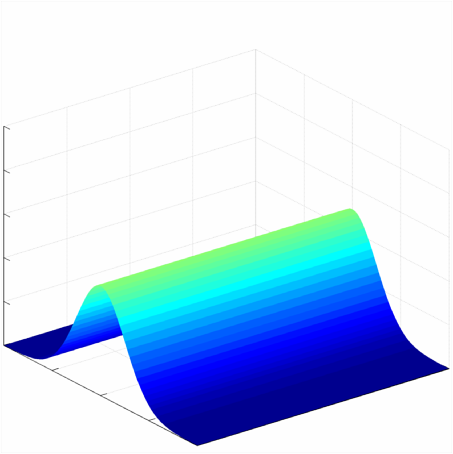
\includegraphics[width=0.2\textwidth]{\additivefigsdir/2d-kernel/additive_kernel_sum_p2} 
& \hspace{-0.4cm} \raisebox{1cm}{+} \hspace{-0.4cm} & 
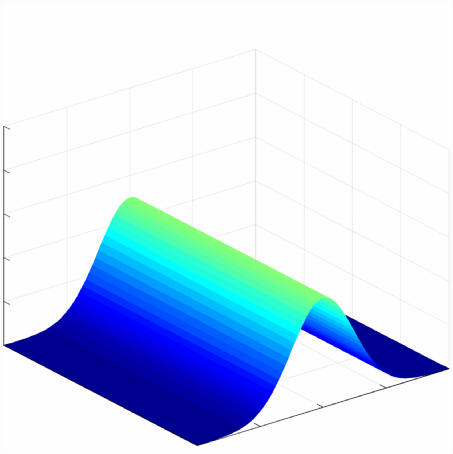
\includegraphics[width=0.2\textwidth]{\additivefigsdir/2d-kernel/additive_kernel_sum_p1} 
& \hspace{-0.4cm} \raisebox{1cm}{=} \hspace{-0.4cm} & 
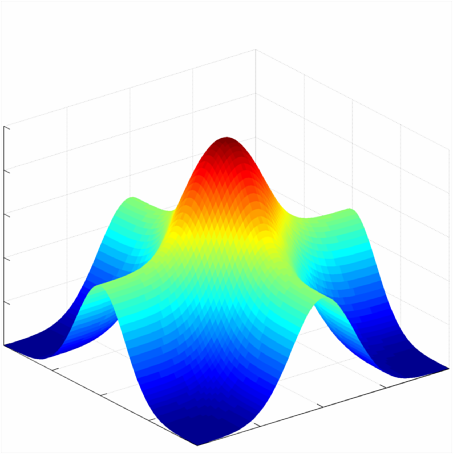
\includegraphics[width=0.2\textwidth]{\additivefigsdir/2d-kernel/additive_kernel} &
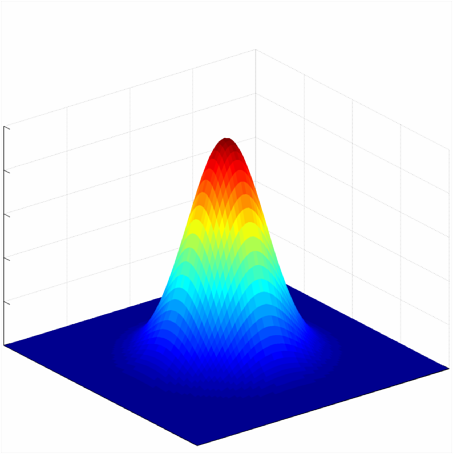
\includegraphics[width=0.2\textwidth]{\additivefigsdir/2d-kernel/sqexp_kernel} \\
$k_1(x_1, x_1')$ & & $k_2(x_2, x_2')$ & & $k_1(x_1,x_1') + k_2(x_2,x_2')$ &$k_1(x_1,x_1')k_2(x_2,x_2')$ \\[1em]
%1D kernel & & 1D kernel & & 1st order kernel & 2nd order kernel \\ 
%& & & & & \\
%(Second Order) & & & & & Additive Kernel \\
%&&&&& \\
\large $\downarrow$ & & \large $\downarrow$ & & \large $\downarrow$ & \large $\downarrow$  \\[-0.2em]
\hspace{-0.2cm}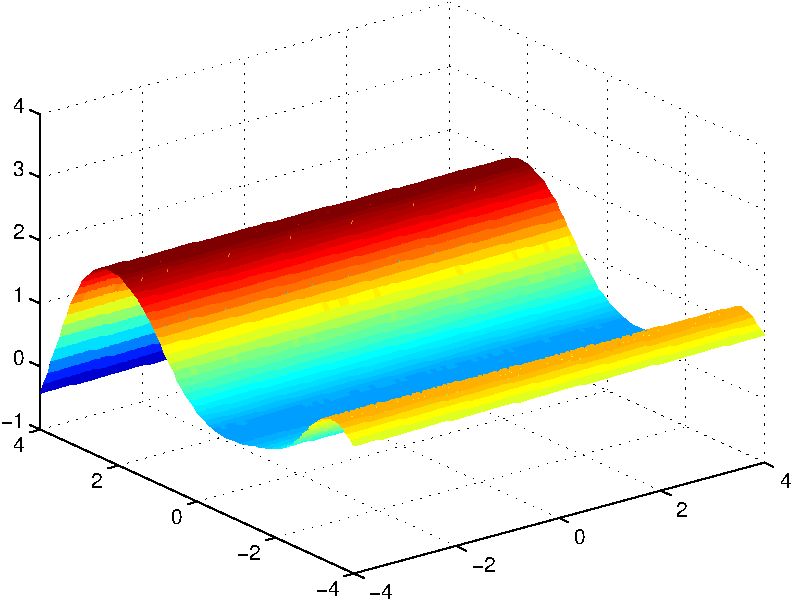
\includegraphics[width=0.2\textwidth]{\additivefigsdir/2d-kernel/additive_kernel_draw_sum_p1}
& \hspace{-0.4cm} \raisebox{1cm}{+} \hspace{-0.4cm} & 
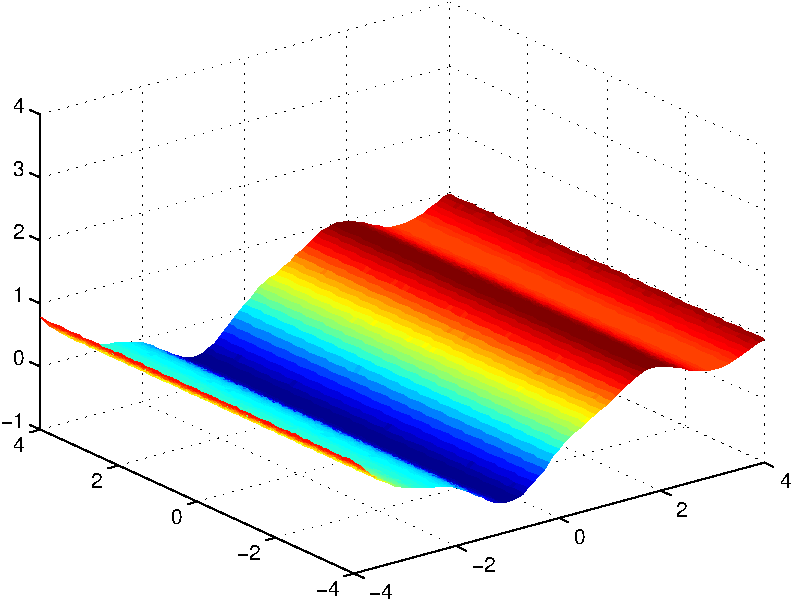
\includegraphics[width=0.2\textwidth]{\additivefigsdir/2d-kernel/additive_kernel_draw_sum_p2}
& \hspace{-0.4cm} \raisebox{1cm}{=} \hspace{-0.4cm} &
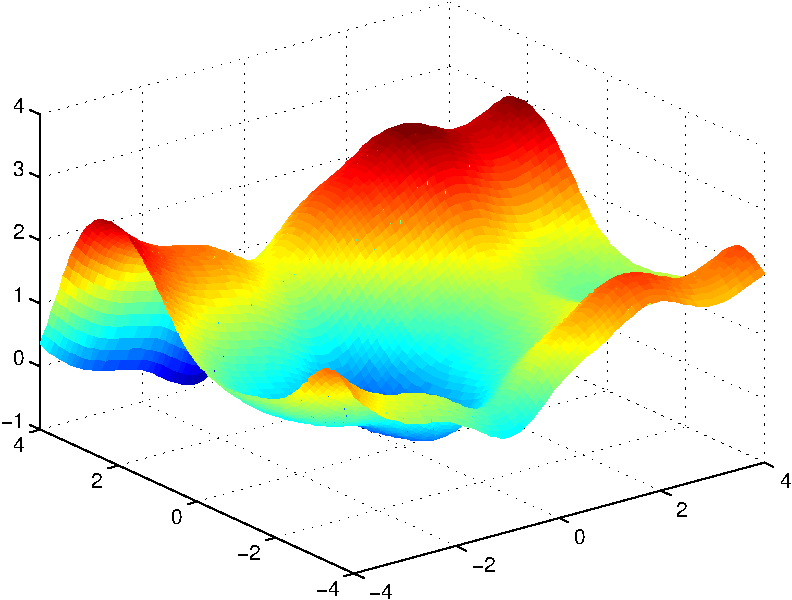
\includegraphics[width=0.2\textwidth]{\additivefigsdir/2d-kernel/additive_kernel_draw_sum} &
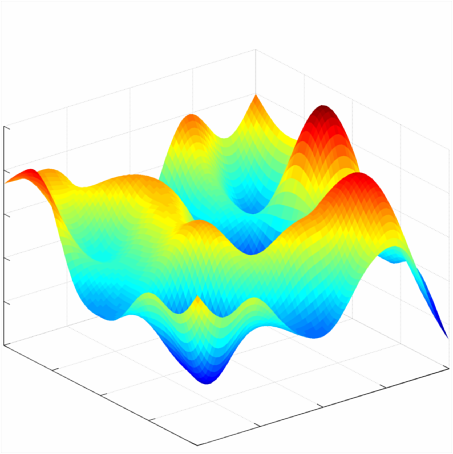
\includegraphics[width=0.2\textwidth]{\additivefigsdir/2d-kernel/sqexp_draw} \\
$f_1 \sim \GP\left(0, k_1\right)$ & & $f_2 \sim \GP\left(0, k_2\right)$ & & $f_1(x_1) + f_2(x_2)$ & $f(x_1, x_2)$ \\
%draw from & & draw from & & draw from & draw from\\
%1D GP prior & & 1D GP prior & & 1st order GP prior & 2nd order GP prior\\
%Draw from product kernel GP prior & Draw from additive kernel GP prior\\
\end{tabular}
\caption[Additive kernels correspond to additive functions]{
\emph{Top left:} An additive kernel is a sum of kernels.
\emph{Bottom left:}  A draw from an additive kernel corresponds to a sum of draws from independent \gp{} priors with the corresponding kernels.
\emph{Top right:} A product kernel.
\emph{Right:}  A \gp{} prior with a product of kernels does not correspond to a product of draws from \gp{}s.
%In this example, both kernels are composed of one dimensional squared-exponential kernels, but this need not be the case in general.
}
\label{fig:kernels}
\end{figure}
%
For example, if
%
\begin{align}
%\function := 
f(x_1, x_2) \dist \GP(\vzero, \kernel_1(x_1, x_1') + \kernel_2(x_2, x_2'))
\end{align}
%
Then this is equivalent to the model
%
\begin{align}
\function_1(x_1) & \dist \GP(\vzero, \kernel_1(x_1, x_1'))\\
\function_2(x_2) & \dist \GP(\vzero, \kernel_2(x_2, x_2'))\\
f(x_1, x_2) & = f_1(x_1) + f_2(x_2)
\end{align}
%
%Then we can model the sum of those functions through another \gp{}:
%

\Cref{fig:kernels} illustrates a decomposition of this form.
Note that the product of two kernels does not have an analogous interpretation as the product of two functions.



\subsection{Example: Additive Model of Concrete Compressive Strength}
\label{sec:concrete}

To illustrate how additive kernels give rise to interpetable models, we'll build an additive model of the strength of concrete as a function of the amount of 7 different ingredients, plus the age of the concrete \citep{yeh1998modeling}.
%We model measurements of the compressive strength of concrete, as a function of the concentration of 7 ingredients, plus the age of the concrete.

Our simple additive model looks like
%
\begin{align}
f(\vx) & = 
f_1(\textnormal{cement}) + f_2(\textnormal{slag}) + f_3(\textnormal{fly ash}) + f_4(\textnormal{water}) \nonumber \\
& \quad + f_5(\textnormal{plasticizer}) + f_6(\textnormal{coarse}) + f_7(\textnormal{fine}) + f_8(\textnormal{age}) + \textnormal{noise}
\label{eq:concrete}
\end{align}
%
where $\textnormal{noise} \simiid \Nt{0}{\sigma_n}$.
After learning the kernel parameters by maximizing the marginal likelihood of the data, we can visualize the predictive distribution of each component of the model.
%
%
\newcommand{\concretepic}[1]{\includegraphics[width=0.31\columnwidth]{\decompfigsdir/concrete-component-#1}}
\newcommand{\concretelegend}[0]{\raisebox{5mm}{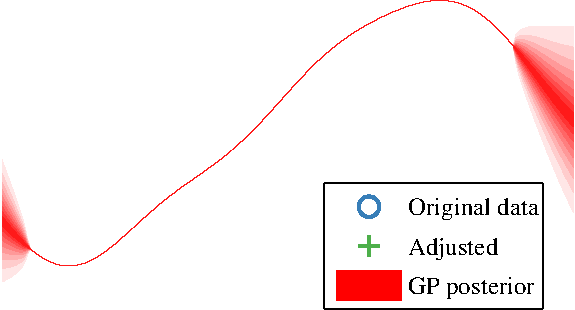
\includegraphics[trim=56mm 1mm 6mm 33mm, clip, width=0.2\columnwidth]{\decompfigsdir/concrete-component-1-legend}}}
%
\begin{figure}[h]
\centering
\begin{tabular}{ccc}
%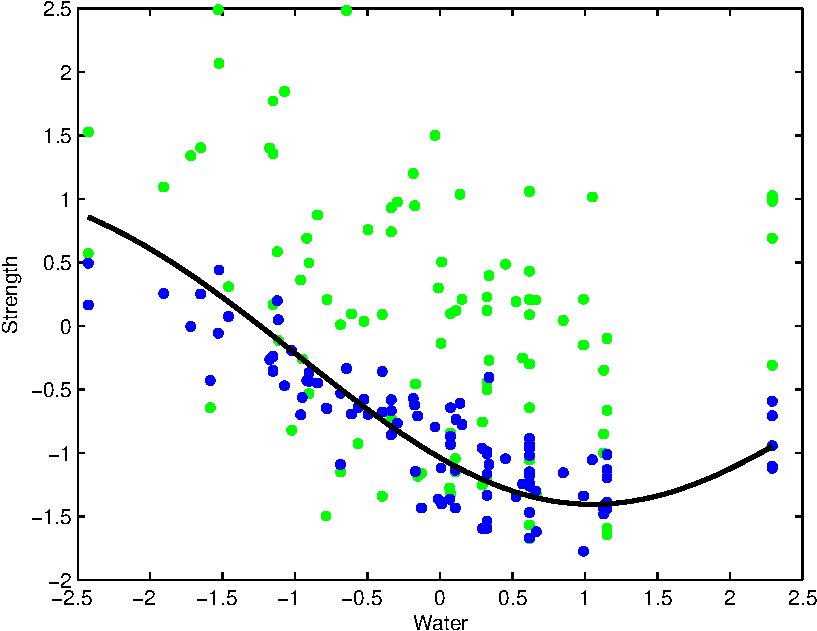
\includegraphics[width=0.3\textwidth]{\additivefigsdir/interpretable_1st_order1.pdf} &
%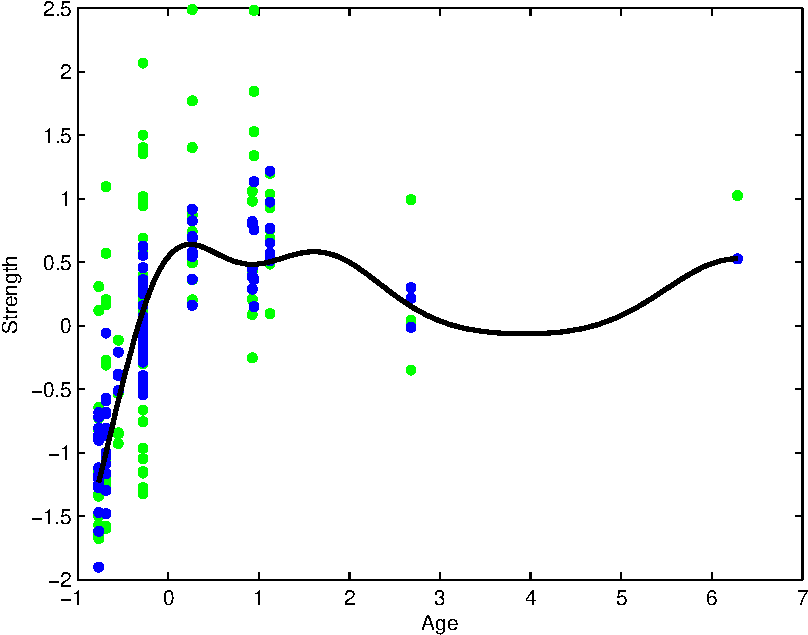
\includegraphics[width=0.3\textwidth]{\additivefigsdir/interpretable_1st_order2.pdf}& 
Cement & Slag & Fly Ash\\
\concretepic{1} & \concretepic{2} & \concretepic{3} \\
 Water & Plasticizer & Coarse\\
\concretepic{4} & \concretepic{5} & \concretepic{6} \\
 Fine & Age \\
 \concretepic{7} & \concretepic{8} & \concretelegend \\
\end{tabular}
\caption[Decomposition of posterior into interpretable one-dimensional functions]
{By considering only one-dimensional terms of the additive kernel, we can plot the predictive distribution of each 1-dimensional function.
Blue points indicate the original data, green points are data after the average contribution from all other terms has been subtracted.
The vertical axis is the same for all plots.
%The black line is the posterior mean of a \sgp{} with only one term in its kernel.
%Right:  the posterior mean of a \sgp{} with only one second-order term in its kernel.
%rs = 1 - var(complete_mean - y)/ var(y)
%R-squared = 0.9094
}
\label{fig:interpretable functions}
\end{figure}
%

\Cref{fig:interpretable functions} shows the marginal posterior distribution of each of the 8 components in \cref{eq:concrete}.
We can see that the parameters controlling the variance of two of the components, Coarse and Fine, were set to zero, meaning that the marginal likelihood preferred a parsimonious model which did not depend on these dimensions.
This is an example of the automatic sparsity that arises by maximizing marginal likelihood in \gp{} models, also known as automatic relevance determination (\ARD) \citep{neal1995bayesian}.
The ability to learn kernel parameters in this way is much more difficult when using non-probabilistic methods such as Support Vector Machines [cite], for which cross-validation is often the best method to select kernel parameters.



\subsection{Posterior Variance of Additive Components}
\label{sec:posterior-variance}


%\footnote{Code is available at \url{github.com/duvenaud/phd-thesis/}}
Here we derive the posterior variance and covariance of all of the additive components of a \gp{}.
These formulas allow us to make plots such as \cref{fig:interpretable functions}.
%These formulas let us plot the marginal variance of each component separately.  These formulas can also be used to examine the posterior covariance between pairs of components.

First, we'll write down the joint prior over the sum of two functions drawn from \gp{} priors.
We'll distinguish between $\vecf(\vX)$ (the function values at the training locations) and  $\vecf(\vX^\star)$ (the function values at some set of query locations).
% so that it's clear which matrices to use to extrapolate.

If $f_1$ and $f_2$ are \emph{a priori} independent, and $f_1 \sim \gp( \mu_1, k_1)$ and $f_2 \sim \gp( \mu_2, k_2)$, then
%
\begin{align}
\left[ \begin{array}{l} 
\vf_1(\vX) \\
\vf_1(\vX^\star) \\
\vf_2(\vX) \\
\vf_2(\vX^\star) \\
\vf_1(\vX) + \vf_2(\vX) \\
\vf_1(\vX^\star) + \vf_2(\vX^\star)
\end{array} \right]
\sim
\Nt{
\left[ \begin{array}{c} \vmu_1 \\ \vmu_1^\star \\ \vmu_2 \\ \vmu_2^\star \\ \vmu_1 + \vmu_2 \\ \vmu_1^\star + \vmu_2^\star \end{array} \right]
}
{\left[ \begin{array}{cccccc} 
\vK_1 & \vK_1^\star & 0 & 0 & \vK_1 & \vK_1^\star \\ 
\vK_1^\star & \vK_1^{\star\star} & 0 & 0 & \vK_1^\star & \vK_1^{\star\star} \\
0 & 0 & \vK_2 & \vK_2^\star & \vK_2 & \vK_2^\star \\ 
0 & 0 & \vK_2^\star & \vK_2^{\star\star} & \vK_2^\star & \vK_2^{\star\star} \\
\vK_1 & \vK_1^\star & \vK_2 & \vK_2^\star & \vK_1 + \vK_2 & \vK_1^\star + \vK_2^\star \\ 
\vK_1^\star & \vK_1^{\star\star}  & \vK_2^\star & \vK_2^{\star\star}  & \vK_1^\star + \vK_2^\star & \vK_1^{\star\star} + \vK_2^{\star\star}\\
\end{array} \right]
}
\end{align}
%
where we represent the Gram matrices, evaluated at all pairs of vectors in bold capitals as ${\vK_{i,j} = k(\vx_i, \vx_j)}$.  So 
%
\begin{align}
\vK_1 & = k_1( \vX, \vX ) \\
\vK_1^\star & = k_1( \vX^\star, \vX ) \\
\vK_1^{\star\star} & = k_1( \vX^\star, \vX^\star )
\end{align}

By the formula for Gaussian conditionals, (given by \cref{eq:gauss_conditional}), we get that the conditional distribution of a \gp{}-distributed function conditioned on its sum with another \gp{}-distributed function is given by
%
\begin{align}
\vf_1(\vX^\star) | \vf_1(\vX) + \vf_2(\vX) \sim \Normal \Big( 
& \vmu_1^\star + \vK_1^{\star\tra} (\vK_1 + \vK_2)\inv \left[ \vf_1(\vX) + \vf_2(\vX) - \vmu_1 - \vmu_2 \right] \nonumber \\
& \vK_1^{\star\star} - \vK_1^{\star\tra} (\vK_1 + \vK_2)\inv \vK_1^{\star} \Big)
%\vf_1(\vx^\star) | \vf(\vx) \sim \mathcal{N}\big( 
%& \vmu_1(\vx^\star) + \vk_1(\vx^{\star}, \vx)  \left[ \vK_1(\vx, \vx) + \vK_2(\vx, \vx) \right]\inv \left( \vf(\vx) - \vmu_1(\vx) - \vmu_2(\vx) \right) , \nonumber \\
%& \vk_1(\vx^{\star}, \vx^{\star}) - \vk_1(\vx^{\star}, \vx)  \left[ \vK_1(\vx, \vx) + \vK_2(\vx, \vx) \right] \inv \vk_1(\vx, \vx^{\star}) 
%\big).
\end{align}
%
These formulae express the model's posterior uncertainty about the different components of the signal, integrating over the possible configurations of the other components.
If we wish to condition on the sum of more than two functions, the term $\vK_1 + \vK_2$ can simply be replaced by $\sum_i \vK_i$ everywhere.




\subsubsection{Posterior Covariance of Additive Components}

\begin{figure}[t]
\centering
\renewcommand{\tabcolsep}{1mm}
\def\incpic#1{\includegraphics[width=0.1\columnwidth]{../figures/decomp/concrete-#1}}
\begin{tabular}{p{2mm}*{6}{c}}
 & {Cement} & {Slag} & {Fly Ash} & {Water} & \parbox{0.1\columnwidth}{Plasticizer} & {Age} \\ 
 \rotatebox{90}{{Cement}} & \incpic{Cement-Cement} & \incpic{Cement-Slag} & \incpic{Cement-Fly-Ash} & \incpic{Cement-Water} & \incpic{Cement-Plasticizer} & \incpic{Cement-Age} \\ 
 \rotatebox{90}{{Slag}} & \incpic{Slag-Cement} & \incpic{Slag-Slag} & \incpic{Slag-Fly-Ash} & \incpic{Slag-Water} & \incpic{Slag-Plasticizer} & \incpic{Slag-Age} \\ 
 \rotatebox{90}{{Fly Ash}} & \incpic{Fly-Ash-Cement} & \incpic{Fly-Ash-Slag} & \incpic{Fly-Ash-Fly-Ash} & \incpic{Fly-Ash-Water} & \incpic{Fly-Ash-Plasticizer} & \incpic{Fly-Ash-Age} \\ 
 \rotatebox{90}{{$\quad$Water}} & \incpic{Water-Cement} & \incpic{Water-Slag} & \incpic{Water-Fly-Ash} & \incpic{Water-Water} & \incpic{Water-Plasticizer} & \incpic{Water-Age} \\ 
 \rotatebox{90}{\parbox{0.1\columnwidth}{Plasticizer}} & \incpic{Plasticizer-Cement} & \incpic{Plasticizer-Slag} & \incpic{Plasticizer-Fly-Ash} & \incpic{Plasticizer-Water} & \incpic{Plasticizer-Plasticizer} & \incpic{Plasticizer-Age} \\ 
 \rotatebox{90}{{Age}} & \incpic{Age-Cement} & \incpic{Age-Slag} & \incpic{Age-Fly-Ash} & \incpic{Age-Water} & \incpic{Age-Plasticizer} & \incpic{Age-Age} \\
 \end{tabular}
 \fbox{
\begin{tabular}{c}
 Correlation \\[1ex]
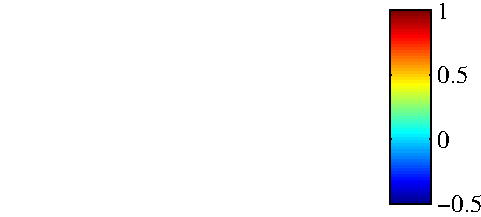
\includegraphics[width=0.1\columnwidth, clip, trim=6.2cm 0cm 0cm 0cm]{../figures/decomp/concrete-colorbar}
\end{tabular}
}
%
%
%
\caption[Visualizing posterior correlations between components]
{Visualizing posterior correlations between the components explaining the concrete dataset.
%Plots on the diagonal show the posterior correlation of each function.
Each plot shows the additive model's posterior correlation between two components, plotted over the domain of the data $\pm 5\%$.
%Color indicates the amount of correlation between the function value of the two components.
Red indicates high correlation, teal indicates no correlation, and blue indicates negative correlation.
%Off-diagonal plots show posterior covariance between each pair of functions, as a function of both inputs.
%Because each
%We can see that t
There is negative correlation between the ``Cement'' and ``Slag'' variables, meaning that - one of these functions is high and the other low, but which one is uncertain under the model.
Dimensions `Coarse' and `Fine' are not shown, because their variance was zero.
}
\label{fig:interpretable interactions}
\end{figure}
%

%One of the advantages of using a generative, model-based approach is that we can examine any aspect of the model we wish to.
We can also compute the posterior covariance between any two components, conditioned on their sum:
%
\begin{align}
\covargs{ \vf_1(\vX^\star)}{\vf_2(\vX^\star) | \vf(\vX) } 
& = - \vK_1^{\star\tra} (\vK_1 + \vK_2)\inv \vK_2^\star
%\covargs{\vf_1(\vx^\star)}{\vf_2(\vx^\star) | \vf(\vx) }
%& = - \vk_1(\vx^{\star}, \vx)  \left[ \vK_1(\vx, \vx) + \vK_2(\vx, \vx) \right] \inv \vk_1(\vx, \vx^{\star}) 
\label{eq:post-component-cov}
\end{align}
%
If this quantity is negative, it means that there is ambiguity about which of the two components explains the data at that location.
\Cref{fig:interpretable interactions} shows the posterior correlation between all non-zero components of the concrete model.
We can see that there is negative correlation between the ``Cement'' and ``Slag'' variables.
This reflects an ambiguity in the model about which one of these functions is high and the other low.



%\subsection{Interpreting Additive Models in High Dimensions}
%As noted by \citet{plate1999accuracy}, o
%One advantage of additive models is their interpretability.
% since a high-dimensional function is decomposed into a series of one- or two-dimensional functions.  
%\citet{plate1999accuracy} demonstrated that by allowing high-order interactions as well as low-order interactions, one can trade off interpretability with predictive accuracy.
%In the case where the kernel parameters indicate that most of the variance in a function can be explained by low-order interactions, it is informative to plot the corresponding low-order functions, as in Figure \ref{fig:interpretable functions}. 




\subsection{Long-range Extrapolation through Additivity}
\label{sec:additivity-extrapolation}

Additive structure often allows us to make predictions far from the training data.
%
\begin{figure}[h!]
\centering
\begin{tabular}{ccc}
 & \gp{} mean using & \gp{} mean using \\
True function: & product of $\kSE$ kernels: & sum of $\kSE$ kernels: \\
\parbox{0.33\columnwidth}{$f(x_1, x_2) = \sin(x_1) + \sin(x_2)$} & $k(x_1, x_1') \times k(x_2, x_2')$ & $k(x_1, x_1') + k(x_2, x_2')$ \\[0.2em]
\hspace{-0.1in}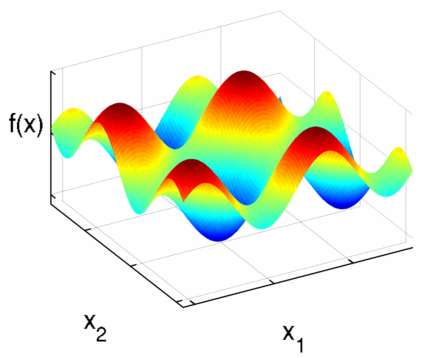
\includegraphics[width=0.32\textwidth]{\additivefigsdir/1st_order_censored_truth} &
\hspace{-0.1in}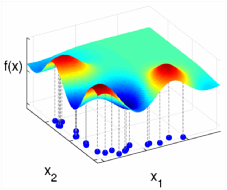
\includegraphics[width=0.32\textwidth]{\additivefigsdir/1st_order_censored_ard}&
\hspace{-0.1in}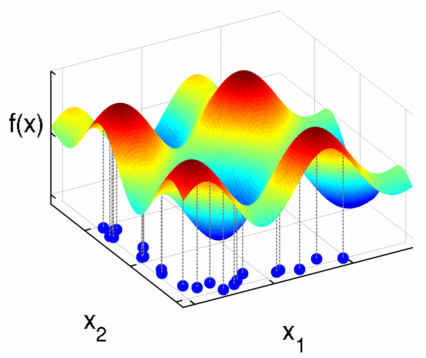
\includegraphics[width=0.32\textwidth]{\additivefigsdir/1st_order_censored_add} \\[1em]
\end{tabular}
\caption[Long-range inference in functions with additive structure]
{Inference in functions with additive structure.
When the function being modeled has additive structure, we can exploit this fact to extrapolate far from the training data.
The product kernel allows a different function value for every combination of inputs, and so is uncertain about function values away from the training data.
%  The additive GP is able to discover the additive pattern, and use it to fill in a distant mode.  The ARD kernel can only interpolate, and thus predicts the mean in locations missing data.
}
\label{fig:synth2d}
\end{figure}
%
Figure \ref{fig:synth2d} compares the extrapolations made by additive versus non-additive \gp{} models, conditioned on data from a sum of two axis-aligned sine functions, evaluated in a small, L-shaped area.
In this example, the additive model is able to correctly predict the height of the function at unseen combinations of inputs.
The product-kernel model is more flexible, and so remains uncertain about the function away from the data.
%The ability of additive GPs to discover long-range structure suggests that this model may be well-suited to deal with covariate-shift problems.

These types of additive models have been well-explored in the statistics literature.  For example, generalized additive models~\citep{hastie1990generalized} have seen wide adoption.
In high dimensions, we can also consider sums of functions of more than one dimension.
\Cref{ch:additive} considers this model class in more detail.






\section{Combining Kernels through Multiplication}

%Multiplying kernels allows us to account for interactions between different input dimensions, or to combine different notions of similarity.

\subsection{Combining High-Level Attributes}

%Loosely speaking, multip

In univariate data, multiplying a kernel by \kSE{} gives a way of converting global structure to local structure.
For example, $\Per$ corresponds to globally periodic structure, whereas $\Per \kerntimes \SE$ corresponds to locally periodic structure, as shown in row 1 of \cref{fig:kernels}.
%
\begin{figure}
\centering
\begin{tabular}{cccc}
$\kLin \times \kLin$ & $\kSE \times \kPer$ & $\kLin \times \kSE$ & $\kLin \times \kPer$ \\
\kernpic{lin_times_lin} & \kernpic{se_times_per} & \kernpic{se_times_lin} & \kernpic{lin_times_per}\\
\fixedx & $x -x'$ & \fixedx & \fixedx\\
%& & & \\
\large $\downarrow$ & \large $\downarrow$ & \large $\downarrow$ & \large $\downarrow$  \\
\kernpic{lin_times_lin_draws}  & \kernpic{se_times_per_draws_s7} & \kernpic{se_times_lin_draws_s2} & \kernpic{lin_times_per_draws_s2} \\
quadratic functions & locally \newline periodic & increasing variation  & growing amplitude \\[10pt]
\end{tabular}
\caption[Examples of one-dimensional structures expressible by multiplying kernels]
{ Examples of one-dimensional structures expressible by multiplying kernels.  
%The x-axis has the same scale for all plots.
Plots have same meaning as in figure \ref{fig:basic_kernels}.}
\label{fig:kernels_times}
\end{figure}

%For instance, in multidimensional data, the multiplicative kernel $\SE_1 \times \SE_2$ represents a smoothly varying function of dimensions 1 and 2 which is not constrained to be additive.

%Since we are applying these operations to the similarity functions rather than the regression functions %themselves, multiplication of even a few base kernels can express complex relationships in data which do not have a simple parametric form.



\subsection{Building Flexible Multidimensional Models}

%For instance, in multidimensional data, the multiplicative kernel $\SE_1 \kerntimes \SE_2$ represents a smoothly varying function of dimensions 1 and 2 which is not constrained to be additive.

For multivariate data, products of $\kSE$ kernels, having a different lengthscale parameter for each dimension, are called the $\seard$ kernel:
%
\begin{align}
\seard( \vx, \vx')
 = \prod_{d=1}^D \exp \left( -\frac{1}{2} \frac{\left( x_d - x'_d \right)^2}{\ell_d^2} \right)
 = \exp \left( -\frac{1}{2} \sum_{d=1}^D \frac{\left( x_d - x'_d \right)^2}{\ell_d^2} \right)
\end{align}
%
\ARD{} stands for Automatic Relevance Determination, so named because by estimating the lengthscale parameters $\ell_1, \ell_2, \dots, \ell_D$, we are implicitly determining the ``relevance'' of each dimension.
Input dimensions with relatively large lengthscales indicate relatively little variation in the function being modeled along those dimensions.


\section{Changepoints}
A simple example of how multiplication of kernels can give rise to more structure priors is given by chapngepoint kernels.
Changepoints kernels can be defined through addition and multiplication with sigmoidal functions:
%

\begin{align}
%\kCP(\kernel_1, \kernel_2) = \kernel_1 \kerntimes \boldsymbol\sigma \kernplus \kernel_2 \kerntimes \boldsymbol{\bar\sigma}
%\kCP(\kernel_1, \kernel_2) & = \begin{array}{rl} (1-\sigma(x)) & k_2(x,x')(1-\sigma(x')) \\
%  + \sigma(x) & k_1(x,x')\sigma(x') \end{array} \\
\kCP(\kernel_1, \kernel_2)(x,x') & = \sigma(x) k_1(x,x')\sigma(x') + (1-\sigma(x)) k_2(x,x')(1-\sigma(x'))
\label{eq:cp}
\end{align}
%
which can be written in shorthand as
%
\begin{align}
\kCP(\kernel_1, \kernel_2)& = \kernel_1 \kerntimes \boldsymbol\sigma \kernplus \kernel_2 \kerntimes \boldsymbol{\bar\sigma}
\end{align}
where $\boldsymbol\sigma = \sigma(x)\sigma(x')$ and $\boldsymbol{\bar\sigma} = (1-\sigma(x))(1-\sigma(x'))$.

This compound kernel expresses a change from one kernel to another.
The parameters of the sigmoid determine where, and how rapidly, this change occurs.

\begin{figure}[h!]
\centering
\begin{tabular}{rcccc}
 & $\kCP(\kSE, \kPer)$ & $\kCP(\kSE, \kPer)$ & $\kCP(\kSE, \kSE)$ & $\kCP(\kPer, \kPer)$ \\
\raisebox{1cm}{f(x)} & \kernpic{../changepoint/draw_1} & \kernpic{../changepoint/draw_2} & \kernpic{../changepoint/draw_3} & \kernpic{../changepoint/draw_4} \\
& $x$ & $x$ & $x$ & $x$
\end{tabular}
\caption[Draws from changepoint priors]
{Draws from different priors on using changepoint kernels, constructed by adding and multiplying together base kernels with sigmoidal functions.
}
\label{fig:changepoint_examples}
\end{figure}

We can also express a function which changes structure within some interval - a change window - by replacing $\sigma(x)$ with a product of two sigmoids, one increasing and one decreasing.

\subsection{Multiplication by a Known Function}

More generally, we can model an unkown function that's been multiplied by some fixed, known function $a(x)$, by multiplying the kernel by $a(\vx) a(\vx')$.
Formally,
%
\begin{align}
f(\iva) = a(\iva) g(\iva), \quad g \sim \GPdist{g}{\vzero}{k(\iva, \iva')} \quad
\iff
\quad f \sim \GPdist{f}{\vzero}{ a(\iva) k(\iva, \iva') a(\iva')}
\end{align}




\section{Feature Representation}
%
By Mercer's theorem \citep{mercer1909functions},
%Due to \citet{mercer1909functions}, we know that
any positive-definite kernel can be represented as the inner product between a fixed set of features, evaluated at $x$ and at $x'$:
%
\begin{align}
k(\vx, \vx') = \feat(\vx)\tra \feat(\vx')
\end{align}

As a simple example, the squared-exponential kernel ($\kSE$) on the real line has a representation in terms of infinitely many radial-basis functions.
Any stationary kernel (one which only depends on the distance between its inputs) on the real line can be represented by a set of sines and cosines - a Fourier representation \citep{bochner1959lectures}.
In general, the feature representation of a kernel is not unique, and depends on which space $\InputSpace$ is being considered \citep{minh2006mercer}.

In some cases, $\InputSpace$ can even be the infinite-dimensional feature mapping of another kernel.  Composing feature maps in this way leads to \emph{deep kernels}, a topic explored in chapter~\ref{ch:deep-limits}.



\subsection{Relation to Linear Regression}

Suprisingly, \gp{} regression is equivalent to Bayesian linear regression on $\feat(\vx)$:
%
\begin{align}
f(\iva) = \vw\tra \feat(\iva), \quad \vw \sim \N{\vw}{\vzero}{\Sigma} \quad
\iff
\quad f \sim \GPdist{f}{\vzero}{\feat(\iva) \tra \Sigma \feat(\iva)}
\end{align}
%
The link between Gaussian processes, linear regression, and neural networks is explored further in chapter~\ref{ch:deep-limits}.


\subsection{Feature-space view of Combining Kernels}

\def\feata{\va}
\def\featb{\vb}

Many architectures for learning complex functions, such as convolutional networks \cite{lecun1989backpropagation} and sum-product networks \cite{poon2011sum}, include units which compute \texttt{and}-like and \texttt{or}-like operations.
Composite kernels can be viewed in this way too.
A sum of kernels can be understood as an \texttt{or}-like operation: two points are considered similar if either kernel has a high value.
Similarly, multiplying kernels is an \texttt{and}-like operation, since two points are considered similar only if both kernels have high values.


We can also view kernel addition and multiplication as a combination of the features of the original kernels.
%Viewing kernel addition from this point of view, if
For example, if we have two kernels
%
\begin{align}
k_a(\iva, \iva') & = \feata(\iva)\tra \feata(\iva')\\
k_b(\iva, \iva') & = \featb(\iva)\tra \featb(\iva')
\end{align}
%
and we consider their addition, then
%
\begin{align}
k_a(\iva, \iva') + k_b(\iva, \iva)
& = \feata(\iva)\tra \featb(\iva') + \feata(\iva)\tra \featb(\iva') \\
& = \colvec{\feata(\iva)}{\featb(\iva)}\tra \colvec{\feata(\iva')}{\featb(\iva')}
\end{align}
%
meaning that the features of $k_a + k_b$ are the concatenation of the features of each kernel.

We can examine kernel multiplication in a similar way:
%
\begin{align}
k_a(\iva, \iva') \times k_b(\iva, \iva')
& = \left[ \feata(\iva)\tra \feata(\iva') \right] \times \left[ \featb(\iva)\tra \featb(\iva') \right] \\
%& = \left[ \begin{array}{c} \feat_1(\iva) \\ \feat_2(\iva) \end{array} \right]^\tra \left[ \begin{array}{c} \feat_1(\iva') \\ \feat_2(\iva') \end{array} \right]
& = \sum_i a_i(\iva) a_i(\iva') \times \sum_j b_j(\iva) b_j(\iva') \\
& = \sum_i \sum_j a_i(\iva) a_i(\iva') b_j(\iva) b_j(\iva') \\
& = \sum_{i,j} \big[ a_i(\iva) b_j(\iva) \big] \big[ a_i(\iva') b_j(\iva') \big] \\
& = \vecop{ \feata(\iva) \otimes \featb(\iva') } \tra \vecop{ \feata(\iva) \otimes \featb(\iva')} 
\end{align}
%
In other words, the features of $k_a \times k_b$ are just the cartesian product (all possible combinations) of the original two sets of features.
For example, a set of infinitely many Gaussian bumps spread evenly along the real line gives rise to one-dimensional $\kSE$ kernel.
The cartesian product of these features with another set spread along a different dimension gives a tiling of the plane with two-dimensional Gaussian bumps.
This tiling corresponds to a two-dimensional $\kSE$ kernel.






\section{Expressing Symmetries and Invariances}

When modeling functions, encoding known symmetries improves both learning and prediction. 
Many types of symmetry can be enforced through operations on the covariance function.
In this section, we'll look at different ways in which we can encode a given symmetry into a prior on functions.

We'll demonstrate the properties of the resulting models by sampling functions from their priors.
By using these priors to define warpings from $\Reals^2 \to \Reals^3$, we'll also show how to build a nonparametric prior on an open-ended family of topological manifolds, such as cylinders, torii, and M\"{o}bius strips.
% These symmetries can be composed to produce nonparametric priors on functions whose domains have interesting topological structure such as spheres, torii, and M\"{o}bius strips.

% I would cite Pierre Chiche but he hasn't actually published his damn papers.

\citet{ginsbourger2012argumentwise} and \citet{Invariances13} characterized the set of \gp{} priors on functions invariant to given transformations.
They showed that the only way to construct a prior on functions which respect a given invariance is to construct a kernel which respects the same invariance with respect to each of its two inputs.

Formally, given a finite group of operations $G$ to which we wish our function to remain invariant, and $f \sim \GPt{0}{k(\vx,\vx')}$, $f$ is invariant under $G$ if and only if $k(\cdot, \cdot)$ is argumentwise invariant:
%
\begin{align}
k( g(\vx), g(\vx')) = k(\vx, \vx'), \quad \forall \vx, \vx' \in \InputSpace, \quad \forall g, g' \in G
\end{align}

\def\gswitch{G_\textnormal{swap}}

As a simple example, consider the symmetry $f(x, y) = f(y,x)$, or the set of functions invariant to swapping their two arguments.
The elements of the group $\gswitch$ describing this symmetry are
%
\begin{align}
g_1(f(x,y)) & = f(x,y) \qquad \textnormal{(identity)}\\
g_2(f(x,y)) & = f(y,x) \qquad \textnormal{(swap)}
\end{align}
%
However, it might not be clear how to find a kernel obeying these symmetries.


\subsection{Three Recipes for Group Invariance}

Fortunately, for finite groups, there are a few simple ways to transform any kernel into one which is argumentwise invariant to actions under any finite group:
%
%
\begin{figure}
\renewcommand{\tabcolsep}{1.5mm}
\begin{tabular}{ccc}
Additive method & Projection method & Product method \\[0.5ex]
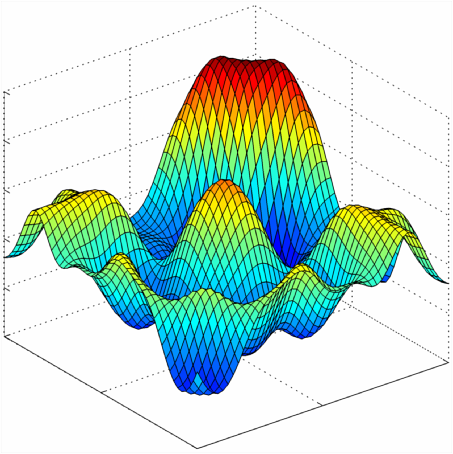
\includegraphics[width=0.3\columnwidth]{\symmetryfigsdir/symmetric-xy-naive-sample} &
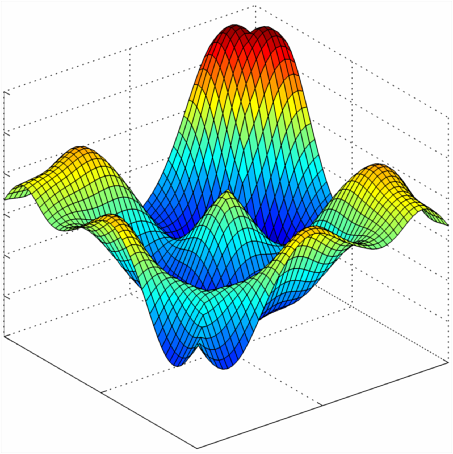
\includegraphics[width=0.3\columnwidth]{\symmetryfigsdir/symmetric-xy-projection-sample} &
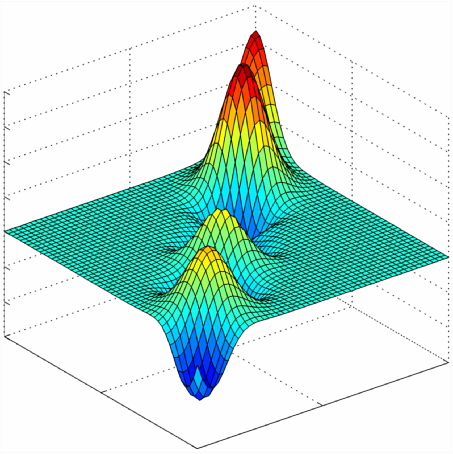
\includegraphics[width=0.3\columnwidth]{\symmetryfigsdir/symmetric-xy-prod-sample}\\
%$k(x, y, x', y') + k(x, y, y', x')$ & $k(x, y, x', y') \times k(x, y, y', x')$ & $k( \min(x, y), \max(x,y),$ \\
% $+ k(y, x, x', y') + k(y, x, y', x')$ & $\times k(y, x, x', y') \times k(y, x, y', x')$ & $\min(x', y'), \max(x',y') )$
$\begin{array}{r@{}l@{}}
& \kSE(x, y, x', y') \\ + & \kSE(x, y, y', x')
\end{array}$
&
$\begin{array}{r@{}l@{}}
\kSE( \!\! &{}\min(x, y), \max(x,y), \\
           &{}\min(x', y'), \max(x',y') )
\end{array}$
&
$\begin{array}{r@{}l@{}}
& \kSE(x, y, x', y') \\ \times & \kSE(x, y, y', x') 
\end{array}$
\end{tabular}
\caption[Three ways to introduce symmetry]{Three methods of introducing symmetry, illustrated through draws from the corresponding priors.
%Left:  The additive method.
%Center: The product method.
%Right: The projection method.
%The additive method has half the marginal variance away from $y = x$, but the min method introduces a non-differentiable seam along $y = x$.
All three methods introduce a different type of nonstationarity.
}
\label{fig:add_vs_min}
\end{figure}
%
\begin{enumerate}

\item {\bf Sum over the Orbit.} 
\citet{ginsbourger2012argumentwise} and \citet{kondor2008group} suggest a double sum over the orbits of $\vx$ and $\vx'$ w.r.t. G:
%
\begin{align}
k_\textnormal{sum}(\vx, \vx') = \sum_{g, \in G} \sum_{g' \in G} k( g( \vx ), g'( \vx') )
\end{align}

For our example group $\gswitch$, this operation results in the kernel:
%
\begin{align}
k_\textnormal{switch}(\vx, \vx')
& = \sum_{g, \in \gswitch} \sum_{g' \in \gswitch} k( g( \vx ), g'( \vx') ) \\
& = k(x, y, x', y') + k(x, y, y', x') + k(y, x, x', y') + k(y, x, y', x')
\end{align}
%
For stationary kernels, some pairs of elements in this sum will be identical, and can be ignored.
\Cref{fig:add_vs_min}(a) shows a draw from a \gp{} prior with an $\kSE$ kernel symmetrized in this way.
This construction has the property that the marginal variance is doubled near $x = y$, which may or may not be desirable.



\item {\bf Project onto a Fundamental Domain.}
\citet{Invariances13} also explore the possibility of projecting each datapoint into a fundamental domain of the group, using a mapping $A_G$:
%
\begin{align}
k_\textnormal{rep}(\vx, \vx') = k( A_G(\vx), A_G( \vx') )
\end{align}
%
For our example group $\gswitch$, a fundamental domain is $\{x, y : x < y\}$, which can be mapped to using $A_{\gswitch}( x, y ) = \big[ \min(x,y), \max(x,y) \big]$.
Constructing a kernel using this method introduces a non-differentiable  ``seam'' along $x = y$, as shown in \cref{fig:add_vs_min}(b).
The projection method also works for infinite groups, as we shall see below.

\item {\bf Multiply over the Orbit.}
Ryan P. Adams (personal communication) suggests a construction using products over the orbits:
%
\begin{align}
k_\textnormal{sum}(\vx, \vx') = \prod_{g, \in G} \prod_{g' \in G} k( g( \vx ), g'( \vx') )
\end{align}
%
This method will often produce \gp{} priors with zero variance in some regions of the space, as in \cref{fig:add_vs_min}(c).
%We include it here to show that each of these methods for enforcing symmetries modifies the resulting model in other ways as well.
\end{enumerate}

There are many possible ways to achive a given symmetry, but we must be careful to do so without compromising other qualities of the model we are constructing.
For example, simply setting $k(\vx, \vx') = 0$ gives rise to a \gp{} prior which obeys \emph{all possible} symmetries, but this is presumably not a model we wish to use.




%In this section, we give recipes for expressing several classes of symmetries.  Later, we will show how these can be combined to produce more interesting structures.


\subsection{Periodicity}

%We can enforce periodicity on any subset of the dimensions:
Periodicity in a one-dimensional function corresponds to the invariance
%
\begin{align}
f(x) = f( x + \tau)
\label{eq:periodic_invariance}
\end{align}
%
where $\tau$ is the period.

The most popular method for building a periodic kernel is due to \citet{mackay1998introduction}, who used the projection method in combination with an $\kSE$ kernel.
A fundamental domain of the symmetry group is a circle, so the kernel
%
%The representer transformation for periodicity is simply $A(x) = [\sin(x), \cos(x)]$:
%
\begin{align}
\kPer(x, x') = \kSE \left( \big[ \sin(x), \cos(x) \big], \big[ \sin(x'), \cos(x') \big] \right)
\end{align}
%
%We can also apply rotational symmetry repeatedy to a single dimension.
achieves the invariance in Equation~\eqref{eq:periodic_invariance}.
Simple algebra reduces this kernel to the form shown in Table~\ref{fig:basic_kernels}.

We could also build a periodic kernel with period $\tau$ by the mapping $A(x) = \mod(x, \tau)$.
However, samples from this prior would be discontinuous at every integer multiple of $\tau$.

\subsection{Reflective Symmetry Along an Axis}

We can enforce symmetry about zero
%
\begin{align}
f(x) = f( -x)
\end{align}
%
using the sum over orbits method, by the transform
%
\begin{align}
k_{\textnormal{symm axis}}(x, x') & = k(x, x') + k(x, -x') + k(-x, x') + k(-x, -x')
\end{align}


%\paragraph{Spherical Symmetry}

%We can also enforce that a function expresses the symmetries obeyed by $n-spheres$ by simply transforming a set of $n - 1$ coordinates by:
%
%\begin{align}
%x_1 & = \cos(\phi_1) \nonumber \\
%x_2 & = \sin(\phi_1) \cos(\phi_2) \nonumber \\
%x_3 & = \sin(\phi_1) \sin(\phi_2) \cos(\phi_3) \nonumber \\
%& \vdots \nonumber \\
%x_{n-1} & = \sin(\phi_1) \cdots \sin(\phi_{n-2}) \cos(\phi_{n-1}) \nonumber \\
%x_n & = \sin(\phi_1) \cdots \sin(\phi_{n-2}) \sin(\phi_{n-1})
%\end{align}

%\cite{flanders1989}



\subsection{Translation Invariance in Images}

Most models of images are invariant to spatial translations \citep{lecun1995convolutional}.
Similarily, most models of sounds are also invariant to translation through time.

This sort of translation-invariance is completely distinct from the stationarity of kernels such as $\kSE$ or $\kPer$.
A stationary kernel implies that the prior is invariant to translations of the entire training and test set.
In contrast, we are discussing here a discretized input space (into pixels or the audio equivalent), where the input vectors have one dimension for each pixel.
We are interested in creating priors on functions that are invariant to shifting a signal along its pixels:
%
\begin{align}
f \Bigg( \raisebox{-2.5ex}{ 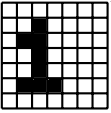
\includegraphics[width=1cm]{\topologyfiguresdir/grid2} } \Bigg) 
= f \Bigg( \raisebox{-2.5ex}{ 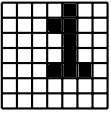
\includegraphics[width=1cm]{\topologyfiguresdir/grid3} } \Bigg)
\end{align}
%
In this setting, translation is equivalent to swapping dimensions of the input vector $\vx$.
For example, in a one-dimensional image, translation could be define as
%
\begin{align}
\shift(\vx, i) = \big[ x_{\mod( i + 1, D )}, x_{\mod( i + 2, D )}, \dots, x_{\mod( D + i, D )} \big]
\end{align}
%
The extension to two dimensions is straightforward, but notationally cumbersome.

Translation invariance in one dimension can be achieved by the transformation
%
\begin{align}
%k \left( (x_1, x_2, \dots, x_D ), (x_1', x_2', \dots, x_D' ) \right) & = %\nonumber \\
%\sum_{i=1}^D \prod_{j=1}^D k( x_j, x_{ i + j \textnormal{mod $D$} }' )
k_\textnormal{invariant} \left( \vx, \vx' \right) = %\nonumber \\
\sum_{i=1}^D \sum_{j=1}^D k( \shift(\vx, i), \shift(\vx, j) )
\end{align}
%
We are simply defining the covariance between two images to be the sum of all covariances between all translations of the two images.

\citet{kondor2008group} built a more elaborate kernel between images, approximately invariant to both translation and rotation by using the projection method.

%Is there a pathology of the additive construction that appears in the limit?

%\subsection{Max-pooling}
%What we'd really like to do is a max-pooling operation.  However, in general, a kernel which is the max of other kernels is not PSD [put counterexample here?].  Is the max over co-ordinate switching PSD?





\section{Generating Topological Manifolds}
\label{sec:topological-manifolds}

We now give a geometric illustration of the symmetries encoded by different combinations of kernels.

Priors on functions exhibiting symmetries can be used to create a prior on topological manifolds, by warping a latent surface $\vx$ to an observed surface $\vy = f(\vx)$.
%The distribution on $\vf$ allows us to put mass on 
%If we set the input $\vx$ to be a 2-dimensional plane, intro 3 dimensions using a \gp{} encoding certain symmetries, the resulting surfaces will correspon
To build a prior on 2-dimensional manifolds embedded in 3-dimensional space, we simply need a prior on mappings from $\mathbb{R}^2$ to $\mathbb{R}^3$, which we can construct using 3 independent functions $[f_1(\vx), f_2(\vx), f_3(\vx)]$ mapping from $\mathbb{R}^2$ to $\mathbb{R}$, specified with \gp{} priors.
%Next, draw 3 independent functions from a \gp{} prior.
% with the relevant symmetries encoded in the kernel.  
%Then, map the 2D mesh through those functions to get 3D coordinates of each point on the mesh.
%[TODO: flesh this out]
Symmetries in $[f_1, f_2, f_3]$ will connect different parts of the manifolds, giving rise to non-trivial topologies on the sampled surfaces.

This construction is similar in spirit to the \gp{} latent variable model (\gplvm{}) of \citet{lawrence2005probabilistic}, which learns a latent embedding of the data into a low-dimensional space, given a \gp{} prior on the mapping from the latent space to the observed space.%and constructs a fixed kernel structure over that space.
%The GP-LVM will be discussed in further detail in chapter ...

%\subsection{Surfaces, Cylinders and Torii}

\begin{figure}
\renewcommand{\tabcolsep}{1mm}
\begin{tabular}{ccc}
Manifold $( \SE_1 \times \SE_2 )$  & Cylinder $( \SE_1 \times \Per_2 )$ & Toroid $( \Per_1 \times \Per_2 )$\\
\hspace{-0.5cm}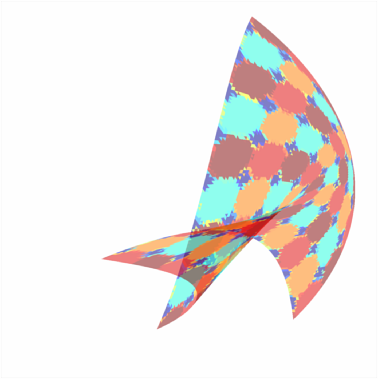
\includegraphics[width=0.33\columnwidth]{\topologyfiguresdir/manifold} &
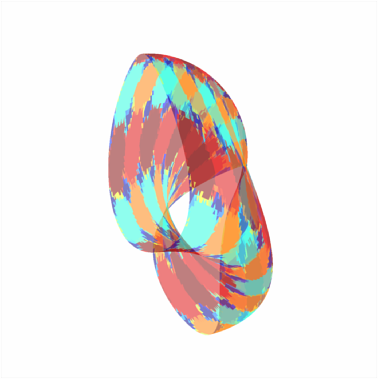
\includegraphics[width=0.33\columnwidth]{\topologyfiguresdir/cylinder} &
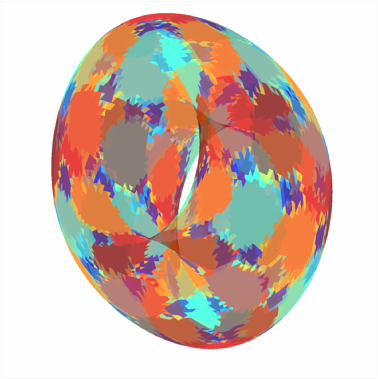
\includegraphics[width=0.33\columnwidth]{\topologyfiguresdir/torus} \\
\end{tabular}
\caption[Generating 2D manifolds with different topological structures]{
Generating 2D manifolds with different topological structures.
By enforcing that the functions mapping from $\mathbb{R}^2$ to $\mathbb{R}^3$ obey the appropriate symmetries, the surfaces created have the corresponding topologies (ignoring self-intersections).
}
\label{fig:gen_surf}
\end{figure}

Figure \ref{fig:gen_surf} shows 2D meshes warped into 3D by functions drawn from \gp{} priors with different kernels.
The different kernels give rise to different topologies.


\subsection{M\"{o}bius Strips}

A prior on functions on M\"{o}bius strips can be achieved by enforcing the symmetries:
%
\begin{align}
f(x, y) & = f( x, y + \tau_y) \\
f(x, y) & = f( x + \tau_x, y)  \\
f(x, y) & = f( y, x )
\end{align}

If we imagine moving along the edge of a M\"{o}bius strip, that is equivalent to moving along a diagonal in the function generated.
Figure~\ref{fig:mobius}a shows an example of a function drawn from such a prior.
%
\begin{figure}
\begin{tabular}[t]{ccc}
%\begin{columns}
\centering
Draw from \gp{} prior: &  &  \\
%$( \Per_1 \times \Per_2 )$ and $f(x,y) = f(y,x)$ & generated parametrically\\
$\begin{array}{l@{}l@{}}
&\Per(x_1, x_1') \kerntimes \Per(x_2, x_2') \\
          \kernplus & \Per(x_1, x_2') \kerntimes \Per(x_2, x_1')
\end{array}$
& $\begin{array}{c} \textnormal{ M\"{o}bius strip}  \\ \textnormal{drawn from manifold prior}  \end{array}$
 & $\begin{array}{c} \textnormal{Sudanese M\"{o}bius strip}  \\ \textnormal{generated parametrically}  \end{array}$\\
%$ + \Per(x_1, x_2') \times \Per(x_2, x_1')$ & \\
%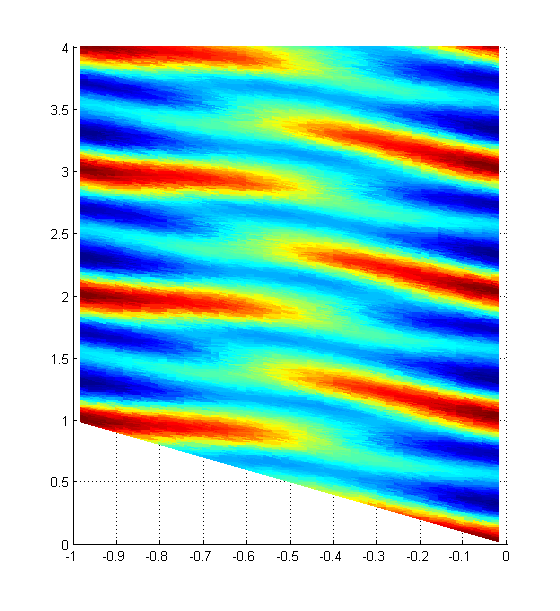
\includegraphics[width=0.45\columnwidth, height=0.45\columnwidth, clip=true,trim=2cm 2cm 2cm 1cm]{\topologyfiguresdir/mobius_regression} \\
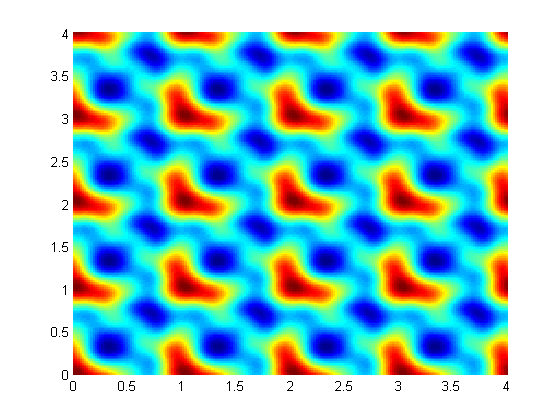
\includegraphics[width=0.3\columnwidth, height=0.3\columnwidth, clip=true,trim=3cm 2cm 2cm 2cm]{\topologyfiguresdir/mobius_field} & 
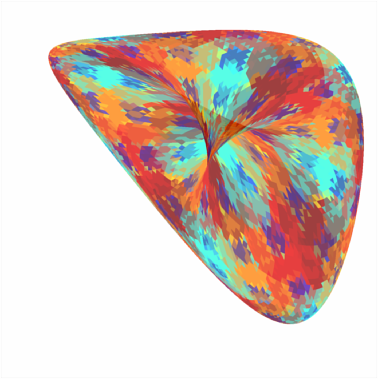
\includegraphics[width=0.3\columnwidth,clip=true,trim=1cm 0cm 0cm 0cm]{\topologyfiguresdir/mobius} &
%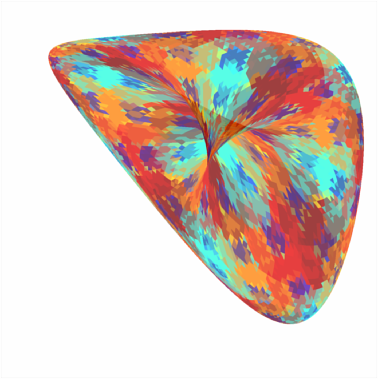
\includegraphics[width=0.33\columnwidth]{\topologyfiguresdir/mobius} 
%\begin{minipage}{0.33\columnwidth}
%{\begin{tabular}[t]{p{.3\columnwidth}}
%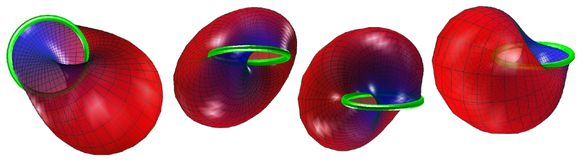
\includegraphics[width=0.3\columnwidth,clip=true,trim=0cm 0cm 10cm 0cm]{\topologyfiguresdir/sudanese-wikipedia}
%\\
%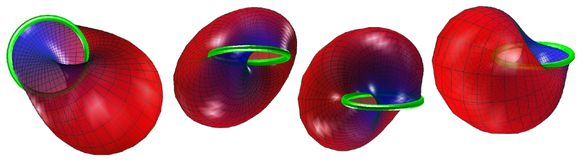
\includegraphics[width=0.3\columnwidth,clip=true,trim=10.55cm 0cm 0cm 0cm]{\topologyfiguresdir/sudanese-wikipedia}
%\end{tabular}}
%\end{minipage}
\raisebox{1cm}{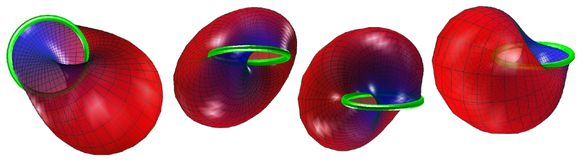
\includegraphics[width=0.25\columnwidth,clip=true,trim=0cm 0cm 14.6cm 0cm]{\topologyfiguresdir/sudanese-wikipedia}}
\end{tabular}
\caption[Generating M\"{o}bius strips]{Generating M\"{o}bius strips.
\emph{Left:} A function drawn from a \sgp{} prior obeying the same symmetries as a M\"{o}bius strip.
\emph{Center:} By enforcing that the functions mapping from $\mathbb{R}^2$ to $\mathbb{R}^3$ obey the appropriate symmetries, surfaces sampled from the prior have topology corresponding to a M\"{o}bius strip.
M\"{o}bius strips generated this way do not have the familiar shape of a circular flat surface with a half-twist; instead they tend to look like \emph{Sudanese} M\"{o}bius strips \citep{sudanese1984}, whose edge has a circular shape.
\emph{Right:} A Sudanese projection of a M\"{o}bius strip.
Image adapted from \citep{sudanesepict}.
}
\label{fig:mobius}
\end{figure}
%
Figure~\ref{fig:mobius}b shows an example of a 2D mesh mapped to 3D by functions drawn from such a prior.
This surface doesn't resemble a typical M\"{o}bius strip, because the edge of the mobius strip is in roughly circular shape, as opposed to the double-loop that one obtains by gluing a strip of paper with a single twist.
The surface shown resembles the Sudanese M\"{o}bius strip \citep{sudanese1984}, shown in Figure~\ref{fig:mobius}c.

%Another classic example of a function living on a Mobius strip is the auditory quality of 2-note intervals.  The harmony of a pair of notes is periodic (over octaves) for each note, and the 



\section{Kernels on Categorical Variables}

%Kernels can be defined over all types of data structures: Text, images, matrices, and even kernels . Coming up with a kernel on a new type of data used to be an easy way to get a NIPS paper.

%\subsection{}

%There is a simple way to do \gp{} regression over categorical variables:
One flexible way to build a kernel over categorical variables is simply to represent your categorical variable by a one-of-k encoding.
For example, if $x \in \{ 1, 2, 3, 4, 5 \}$, $\oneofk(3) = [0, 0, 1, 0, 0]$.
%For example, if your number ranges from 1 to 5, represent that as 5 different data dimensions, only one of which is on at a time. 
%
\begin{align}
k_{\textnormal{categorical}}( x, x') = \seard( \oneofk(x), \oneofk(x') )
\end{align}
%
Short lengthscales for any particular dimension in the $\seard$ kernel indicate that that category is dissimilar to all others.

A more flexible parameterization suggested by Kevin Swersky (personal communication) allows complete flexibility about which pairs of categories are similar to one another, replacing the $\seard$ kernel with the fully-parameterized $\sefull$:
%
\begin{align}
\sefull( \vx, \vx') = \exp \left( -\frac{1}{2} \vx\tra \vL \vx' \right)
\end{align}
%
where $L$ is symmetric.  This kernel individually parameterizes the covariance between each pair of categories.

%Then, simply put a product of kernels on those dimensions.
%This is the same as putting one SE ARD kernel on all of them.
%Learning the lengthscale on each dimension of the $\kSE$ kernel will now encode how similar the value of the different categories are to one another.
%The lengthscale hyperparameter will now encode whether, when that coding is active, the rest of the function changes.
%If you notice that the estimated lengthscales for your categorical variables is short, your model is saying that it's not sharing any information between data of different categories. 









\iffalse

\section{Worked example: building a structured kernel for a time-series}

%\subsection{Modeling multiple periodicities}

\begin{figure}[h]
\begin{tabular}{ccc}
Long-term trend & Weekly periodicity &Yearly periodicity \\
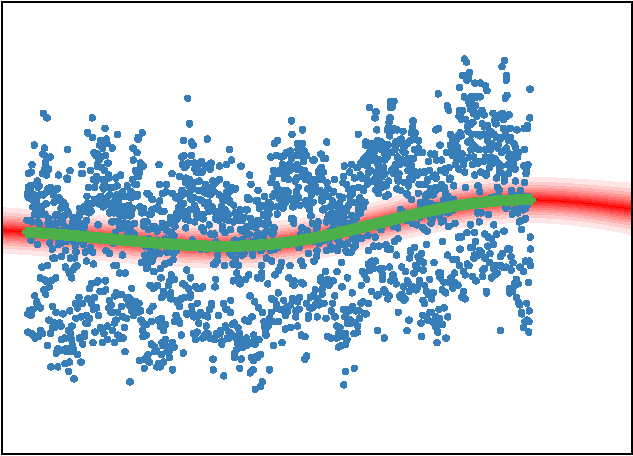
\includegraphics[width=0.31\columnwidth]{\examplefigsdir/births-component-1} &
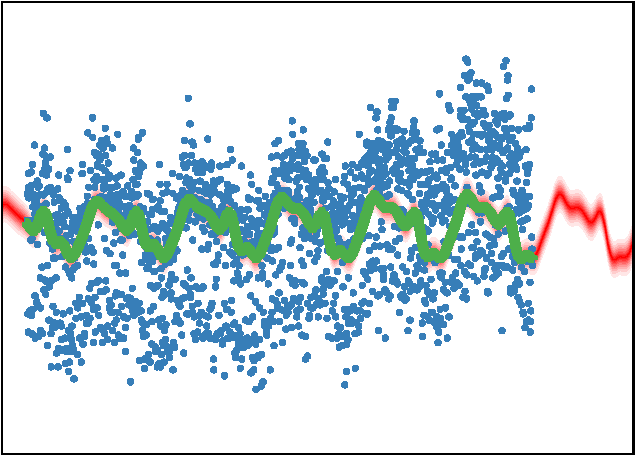
\includegraphics[width=0.31\columnwidth]{\examplefigsdir/births-component-3} & 
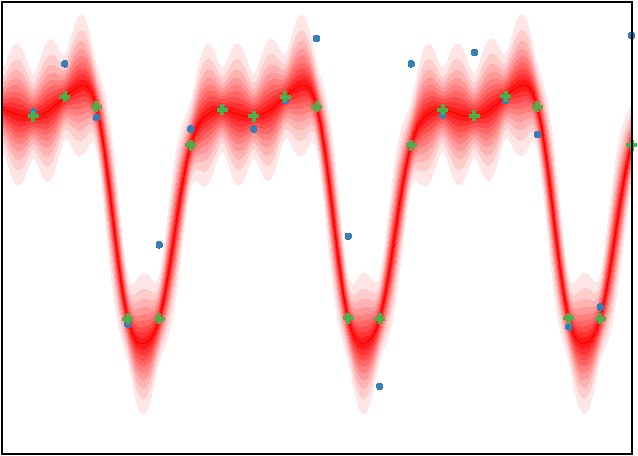
\includegraphics[width=0.31\columnwidth]{\examplefigsdir/births-component-2-zoom} 
\end{tabular}
\caption[Composite model of births data]{A composite \gp{} model of births data. (blue)}
\label{fig:quebec-decomp}
\end{figure}





\iffalse
\begin{figure}
\renewcommand{\tabcolsep}{1mm}
\def \incpic#1{\includegraphics[width=0.200\columnwidth]{../figures/worked-example/births-#1}}
\begin{tabular}{*{5}{c}}
 & {Long-term} & {Weekly} & {Yearly} & {Short-term} \\ 
 \rotatebox{90}{{Long-term}} & \incpic{Long-term-Long-term} & \incpic{Long-term-Weekly} & \incpic{Long-term-Yearly} & \incpic{Long-term-Short-term} \\ 
 \rotatebox{90}{{Weekly}} & \incpic{Weekly-Long-term} & \incpic{Weekly-Weekly} & \incpic{Weekly-Yearly} & \incpic{Weekly-Short-term} \\ 
 \rotatebox{90}{{Yearly}} & \incpic{Yearly-Long-term} & \incpic{Yearly-Weekly} & \incpic{Yearly-Yearly} & \incpic{Yearly-Short-term} \\ 
 \rotatebox{90}{{Short-term}} & \incpic{Short-term-Long-term} & \incpic{Short-term-Weekly} & \incpic{Short-term-Yearly} & \incpic{Short-term-Short-term} \\ 
 \end{tabular}
\caption[Two-way interactions in births data]{Two-way interactions in births data}
\label{fig:quebec-decomp}
\end{figure}
\fi
%\subsection{Incoportating discrete covariates}

%\subsection{Breaking down the predictions, examining different parts of the model}
\fi






\section{Learning Kernel Parameters}

One difficulty in building \gp{} models is choosing, or integrating over, the kernel parameters.
Fortunately, typical kernels only have $\mathcal{O}(D)$ parameters, meaning that if $N$ is reasonably large, these parameters can be estimated by maximum marginal likelihood.
For a fixed kernel form, these parameters can be optimized by gradient-based methods.


\section{Automatically Choosing a Kernel}

%The marginal likelihood of a model is useful for choosing among parameters.
The marginal likelihood can also be used to select the form of the kernel.

For example, we might not know whether a particular structure or symmetry is present in the function we are trying to model.
%Again, the fact that we can compare marginal likelihoods in \gp{}s means that we can 
%Because \gp{}s let us build models both with and without certain symmetries, 
By building kernels with and without such structure, we can compute the marginal likelihoods of the corresponding \gp{} models.
The quantities represent the relative amount of evidence that the data provide for each of these possibilities, providing the assumptions of the model are correct.
%To do so, we simple need to compare the marginal likelihood of the data
%We demonstrate that marginal likeihood an be used to automatically search over such structures.


\subsubsection{Source Code}
Source code to perform all experiments is available at \url{github.com/duvenaud/pdh-thesis/}. 
All \gp{} parameter optimisation was performed by automated calls to the \GPML{} toolbox, available at \url{www.gaussianprocess.org/gpml/code/}.

\section{Conclusion}

We've seen that kernels are a flexible and powerful language for building models of different types of functions.
However, for a given problem, it can difficult to specify an appropriate kernel, even after looking at the data.
A better procedure would be to compare the predictive performance, or marginal likelihood, of a few different kernels.
However, it might be difficult to enumerate all plausible kernels, and tedious to search over them.
%In fact, choosing the kernel can be considered one of the main difficulties in doing inference.

Analogously, we usually don't expect to simply guess the best value of some parameter.
Rather, we specify a search space and an objective, and ask the computer to the search this space for us. 
In the next chapter, we'll see how to perform such a search an automatic search over the open-ended, discrete space of kernel expressions.


\outbpdocument{
\bibliographystyle{plainnat}
\bibliography{references.bib}
}



\iffalse


\subsection{Example: Computing Molecular Energies}

\begin{figure}
\begin{center}
\begin{tabular}{cc}
Function on M\"{o}bius strip & \\
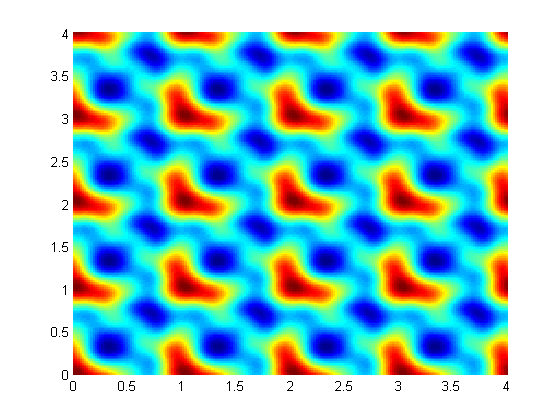
\includegraphics[width=0.3\columnwidth, height=0.3\columnwidth, clip=true,trim=3cm 2cm 2cm 2cm]{\topologyfiguresdir/mobius_field} & 
  \begin{tikzpicture}

%\pgfmathsetmacro{\r}{3cm}
%\pgfmathsetmacro{\ho}{70}
%\pgfmathsetmacro{\ht}{30}
\newcommand{\radius}{3}
\newcommand{\hone}{120}
\newcommand{\htwo}{70}
\newcommand{\hthree}{30}

	\coordinate (O) at (0, 0);
	\coordinate (left) at ({\radius*cos(\hone)}, {\radius*sin(\hone)});
	\coordinate (right) at ({\radius*cos(\htwo)}, {\radius*sin(\htwo)});
	\coordinate (zero) at ({\radius*cos(\hthree)}, {\radius*sin(\hthree)});

	\draw[fill] (left) circle (2pt);
	\draw (left) node[below, left] {H};
	
	\draw[fill] (right) circle (2pt);
	\draw (right) node[right] {H};

	\draw[fill] (zero) circle (2pt);
	\draw (zero) node[right] {H};

	\draw[fill] (O) circle (3pt);
	\draw (O) node[below] {C};

	\draw (left) -- (O);
	\draw (right) -- (O);
	\draw (zero) -- (O);

	\begin{scope}
	\path[clip] (O) -- (right) -- (zero);
	\fill[red, opacity=0.5, draw=black] (O) circle (2);
	\node at ($(O)+(50:1.6)$) {$\theta_1$};	
	\end{scope}
	
	\begin{scope}
	\path[clip] (O) -- (left) -- (right);
	\fill[green, opacity=0.5, draw=black] (O) circle (1.8);
	\node at ($(O)+(90:1.4)$) {$\theta_2$};	
	\end{scope}	
  \end{tikzpicture}
\end{tabular}
\end{center}
\caption[The energy of a molecular configuration obeys the same symmetries as a M\"{o}bius strip]{An example of a function expressing the same symmetries as a M\"{o}bius strip in two of its arguments.  The energy of a molecular configuration $f(\theta_1, \theta_2)$ depends only on the relative angles between atoms, and because each atom is indistiguishable, is invariant to permuting the atoms. }
\label{fig:molecule}
\end{figure}

Figure \ref{fig:molecule} gives one example of a function which obeys the same symmetries as a M\"{o}bius strip, in some subsets of its arguments.

\fi
